% This is "sig-alternate.tex" V2.1 April 2013
% This file should be compiled with V2.5 of "sig-alternate.cls" May 2012
%
% This example file demonstrates the use of the 'sig-alternate.cls'
% V2.5 LaTeX2e document class file. It is for those submitting
% articles to ACM Conference Proceedings WHO DO NOT WISH TO
% STRICTLY ADHERE TO THE SIGS (PUBS-BOARD-ENDORSED) STYLE.
% The 'sig-alternate.cls' file will produce a similar-looking,
% albeit, 'tighter' paper resulting in, invariably, fewer pages.
%
% ----------------------------------------------------------------------------------------------------------------
% This .tex file (and associated .cls V2.5) produces:
%       1) The Permission Statement
%       2) The Conference (location) Info information
%       3) The Copyright Line with ACM data
%       4) NO page numbers
%
% as against the acm_proc_article-sp.cls file which
% DOES NOT produce 1) thru' 3) above.
%
% Using 'sig-alternate.cls' you have control, however, from within
% the source .tex file, over both the CopyrightYear
% (defaulted to 200X) and the ACM Copyright Data
% (defaulted to X-XXXXX-XX-X/XX/XX).
% e.g.
% \CopyrightYear{2007} will cause 2007 to appear in the copyright line.
% \crdata{0-12345-67-8/90/12} will cause 0-12345-67-8/90/12 to appear in the copyright line.
%
% ---------------------------------------------------------------------------------------------------------------
% This .tex source is an example which *does* use
% the .bib file (from which the .bbl file % is produced).
% REMEMBER HOWEVER: After having produced the .bbl file,
% and prior to final submission, you *NEED* to 'insert'
% your .bbl file into your source .tex file so as to provide
% ONE 'self-contained' source file.
%
% ================= IF YOU HAVE QUESTIONS =======================
% Questions regarding the SIGS styles, SIGS policies and
% procedures, Conferences etc. should be sent to
% Adrienne Griscti (griscti@acm.org)
%
% Technical questions _only_ to
% Gerald Murray (murray@hq.acm.org)
% ===============================================================
%
% For tracking purposes - this is V2.0 - May 2012

\documentclass{sig-alternate-05-2015}
\usepackage{subfigure} 
\usepackage{etoolbox}
\makeatletter
\def\@copyrightspace{\relax}
\def\alignauthor{\relax}
\makeatother

\begin{document}

% Copyright
%\setcopyright{acmcopyright}
%\setcopyright{acmlicensed}
%\setcopyright{rightsretained}
%\setcopyright{usgov}
%\setcopyright{usgovmixed}
%\setcopyright{cagov}
%\setcopyright{cagovmixed}


% DOI
%\doi{10.475/123_4}

% ISBN
%\isbn{123-4567-24-567/08/06}

%Conference
%\conferenceinfo{PLDI '13}{June 16--19, 2013, Seattle, WA, USA}

%\acmPrice{\$15.00}

%
% --- Author Metadata here ---
%\conferenceinfo{WOODSTOCK}{'97 El Paso, Texas USA}
%\CopyrightYear{2007} % Allows default copyright year (20XX) to be over-ridden - IF NEED BE.
%\crdata{0-12345-67-8/90/01}  % Allows default copyright data (0-89791-88-6/97/05) to be over-ridden - IF NEED BE.
% --- End of Author Metadata ---

\title{Latency Impact of Docker Containers: A Closer Look
%\titlenote{(Produces the permission block, and
%copyright information). For use with
%SIG-ALTERNATE.CLS. Supported by ACM.}
}
%\subtitle{[Extended Abstract]
%\titlenote{A full version of this paper is available as
%\textit{Author's Guide to Preparing ACM SIG Proceedings Using
%\LaTeX$2_\epsilon$\ and BibTeX} at
%\texttt{www.acm.org/eaddress.htm}}}
%
% You need the command \numberofauthors to handle the 'placement
% and alignment' of the authors beneath the title.
%
% For aesthetic reasons, we recommend 'three authors at a time'
% i.e. three 'name/affiliation blocks' be placed beneath the title.
%
% NOTE: You are NOT restricted in how many 'rows' of
% "name/affiliations" may appear. We just ask that you restrict
% the number of 'columns' to three.
%
% Because of the available 'opening page real-estate'
% we ask you to refrain from putting more than six authors
% (two rows with three columns) beneath the article title.
% More than six makes the first-page appear very cluttered indeed.
%
% Use the \alignauthor commands to handle the names
% and affiliations for an 'aesthetic maximum' of six authors.
% Add names, affiliations, addresses for
% the seventh etc. author(s) as the argument for the
% \additionalauthors command.
% These 'additional authors' will be output/set for you
% without further effort on your part as the last section in
% the body of your article BEFORE References or any Appendices.

%\numberofauthors{8} %  in this sample file, there are a *total*
% of EIGHT authors. SIX appear on the 'first-page' (for formatting
% reasons) and the remaining two appear in the \additionalauthors section.
%
%\author{
%% You can go ahead and credit any number of authors here,
%% e.g. one 'row of three' or two rows (consisting of one row of three
%% and a second row of one, two or three).
%%
%% The command \alignauthor (no curly braces needed) should
%% precede each author name, affiliation/snail-mail address and
%% e-mail address. Additionally, tag each line of
%% affiliation/address with \affaddr, and tag the
%% e-mail address with \email.
%%
%% 1st. author
%\alignauthor
%Ben Trovato\titlenote{Dr.~Trovato insisted his name be first.}\\
%       \affaddr{Institute for Clarity in Documentation}\\
%       \affaddr{1932 Wallamaloo Lane}\\
%       \affaddr{Wallamaloo, New Zealand}\\
%       \email{trovato@corporation.com}
%% 2nd. author
%\alignauthor
%G.K.M. Tobin\titlenote{The secretary disavows
%any knowledge of this author's actions.}\\
%       \affaddr{Institute for Clarity in Documentation}\\
%       \affaddr{P.O. Box 1212}\\
%       \affaddr{Dublin, Ohio 43017-6221}\\
%       \email{webmaster@marysville-ohio.com}
%% 3rd. author
%\alignauthor Lars Th{\o}rv{\"a}ld\titlenote{This author is the
%one who did all the really hard work.}\\
%       \affaddr{The Th{\o}rv{\"a}ld Group}\\
%       \affaddr{1 Th{\o}rv{\"a}ld Circle}\\
%       \affaddr{Hekla, Iceland}\\
%       \email{larst@affiliation.org}
%}
% There's nothing stopping you putting the seventh, eighth, etc.
% author on the opening page (as the 'third row') but we ask,
% for aesthetic reasons that you place these 'additional authors'
% in the \additional authors block, viz.
%\additionalauthors{Additional authors: John Smith (The Th{\o}rv{\"a}ld Group,
%email: {\texttt{jsmith@affiliation.org}}) and Julius P.~Kumquat
%(The Kumquat Consortium, email: {\texttt{jpkumquat@consortium.net}}).}
%\date{30 July 1999}
% Just remember to make sure that the TOTAL number of authors
% is the number that will appear on the first page PLUS the
% number that will appear in the \additionalauthors section.

\maketitle
\begin{abstract}
Traditionally, many web services are held on virtual machines (VMs) provided by cloud computing suppliers. Since VMs bring about dramatic performance degradation compared to bare metal, the quality of service (QoS) is affected. Among all the QoS features, service latency is of crucial importance. With the prevalence of Docker, containers, also called ``lightweight VM'', offer another choice to deploy web applications on the cloud. This paper takes the first to thoroughly analyze the impact of different Docker configurations on service latency. We conclude that the CPU quota configuration might lead to a long tail latency. Docker bridge could lead to a fixed amount of latency degradation instead of a percentage fallen. Using AUFS could bring about extra latency when opening a file or traversing the file system, and have no effect on writing data to a file.
\end{abstract}


%
% The code below should be generated by the tool at
% http://dl.acm.org/ccs.cfm
% Please copy and paste the code instead of the example below. 
%
%\begin{CCSXML}
%<ccs2012>
% <concept>
%  <concept_id>10010520.10010553.10010562</concept_id>
%  <concept_desc>Computer systems organization~Embedded systems</concept_desc>
%  <concept_significance>500</concept_significance>
% </concept>
% <concept>
%  <concept_id>10010520.10010575.10010755</concept_id>
%  <concept_desc>Computer systems organization~Redundancy</concept_desc>
%  <concept_significance>300</concept_significance>
% </concept>
% <concept>
%  <concept_id>10010520.10010553.10010554</concept_id>
%  <concept_desc>Computer systems organization~Robotics</concept_desc>
%  <concept_significance>100</concept_significance>
% </concept>
% <concept>
%  <concept_id>10003033.10003083.10003095</concept_id>
%  <concept_desc>Networks~Network reliability</concept_desc>
%  <concept_significance>100</concept_significance>
% </concept>
%</ccs2012>  
%\end{CCSXML}
%
%\ccsdesc[500]{Computer systems organization~Embedded systems}
%\ccsdesc[300]{Computer systems organization~Redundancy}
%\ccsdesc{Computer systems organization~Robotics}
%\ccsdesc[100]{Networks~Network reliability}


%
% End generated code
%

%
%  Use this command to print the description
%
%\printccsdesc

% We no longer use \terms command
%\terms{Theory}

\keywords{Docker; container; latency; linux bridge; AUFS}

\section{Introduction}

Began from an open-source advanced container engine of dotCloud, a Platform-as-a-Service (PaaS) supplier, Docker is becoming one of the most promising virtualization platform. It significantly shortens the process of packing, shipping and running applications\cite{merkel2014docker}. By packing all the dependencies of the application into several image layers, you can carry the package around and run it with simple commands on almost every laptop, personal computer, and even cloud center as long as running a Linux operating system.

Unlike traditional virtual machines, which use hardware-level virtualization, Docker containers employ system-level virtualization and share the same kernel with the host machine\cite{soltesz2007container}. Many researches\cite{felter2015updated, kratzke2015microservices} have proved that containers have a better performance in most cases than VMs. Due to these performance reasons, many companies are trying to move services from virtual machines to containers\cite{he2012elastic}. However, containers do add additional layers compared to bare-metal hardware, which leads to certain degree of performance degradation.

Docker was born to replace virtual machines to some extent. Nowadays, the widely known Infrastructure-as-a-Service (IaaS) platforms like Amazon EC2 uses virtual machines to run applications like cache and database. Most of these applications not only focus on throughput, but also favor real-time low latency. However, most related work of Docker focus mostly on containers? influence on throughput instead of the latency degradation. Since Docker provides many choices of resource isolation, in this paper, we will do research on how these parameters will affect the latency performance of real time applications.

\subsection{Motivation}

Many modern web services like Google and Facebook are interactive. Responses should be returned very soon otherwise users might complain. Also, these services are dynamic. Data centers process huge amount of data based on the user input and response in very limited time. For example, it requires thousands of Memcached machines to do a simple request through Facebook servers\cite{nishtala2013scaling} and tens of thousands of index servers to do a Bing search\cite{jalaparti2013speeding}. In these cases, not only the throughput is of crucial importance to serve as many clients as possible concurrently, latency should also be taken into account to provide users with the best interactivity. Each additional time cost in one of the service backend layers would increase the overall latency. If all of these separated services require software virtualization layer, a millisecond's latency might be amplified to several thousand milliseconds, thus greatly influencing the overall performance of the service.

Tail latency is another issue to care about\cite{dean2013tail}. In Map-Reduce task\cite{dean2008mapreduce}, a program is processed by hundreds of machines. The result of each map machine is passed to a central reduce machine, so the reduce one has to wait all map ones before moving on. In this case, a map work done over one minute encumbers the whole system even if others are finished in several seconds. Assume that a task has one hundred sub tasks and each sub task has a 99\% probability to finish in one microsecond while 1\% to finish over 1 second. Then the overall performance of this job is 63.3\% probability to finish over one second, which is a rather bad performance. The one-in-one-thousand situation becomes a common case.

The CTO of GigaSpaces claimed a list of interesting phenomenons. He pointed out that latency is a serious matter that can lead to huge profit lost in many companies. Every 100ms of latency would cost Amazon 1\% of lost in sales. Also, every extra of 0.5 seconds wasted on generating a search page can drop Google's network traffic 20\%. Moreover, if a broker's electronic trading platform can not catch up others and gets 5 milliseconds behind the competition, they would lose \$4 million in revenues per millisecond. Even these latencies seems relatively small, people hate waiting. They feel repulsed by these less interactive services, quickly click away and finally do other thing, like turning to the opponents' services. People are talking about how to scaling up the capacity of their services, but they sometimes neglect the importance of building low-latency ones. Service suppliers should try their best to decrease service latency, increase interactivity, and finally lower the customer defection rate\cite{colgate1996customer}.

Despite the increasing need of virtualization technologies to decrease latency, Docker doesn't seem to be focusing on this part. In fact, although Docker provides us a simple way to deploy applications, the technologies it employs are not so latency-friendly. Like what has been mentioned in IBM's technical report\cite{felter2015updated}, Docker containers take the Linux bridge as the method of network isolation. However, it shows that Docker containers even perform worse in transmission throughput and also have a longer network latency compared to KVM\cite{kivity2007kvm}. Actually, all technologies used by Docker are not new ones. Most of them have already existed since the year of 2007, and the concept of container also occurs at that time\cite{soltesz2007container}. Docker container is just a combination of these simple technologies. With the concept of Docker images and the emergence of Docker Hub, Docker quickly win the eyes of system deployers. However, since most of these technologies are provided by old versions of Linux Kernel and they focus on resource isolation instead of latency, it will take Docker a long time to find ways to replace those inefficient technologies and thus decreasing latency lost.

Unlike Google or Facebook, which has dedicated data centers for their services, most small companies cannot afford the cost of hardware and the following mantaince. They can only deploy services on cloud centers like Amazon EC2. As we have mentioned above, these cloud centers use virtual machines to provide hardware virtualization and has a significant performance cost compared to bare metal. The occurrence of Docker thus provide another choice for these customers. Many cloud center service suppliers like Amazon EC2\cite{amazon2010amazon} and Microsoft Azure\cite{copeland2015overview} provide container services in recent years. To simplify the deployment of applications, these small companies are considering to use Docker cloud. Since the additional layer of virtual machine brings about significant performance lost\cite{huber2011evaluating} and is part of the source reason of long latency, it is very important for them to know the trade off between the convenience and latency performance degradation of using Docker to deploy latency-sensitive applications.

Previous researches mainly focus on throughput of CPU, memory and I/O. Some of them talks about memory footprint and the latency bring about by Docker network bridge and methods to shorten this latency. However, these methods are not suitable for public cloud. This paper intended to solve the problem from the customers perspective. Although customers can not the change the services provide by cloud service suppliers, they have the choice to choose their start up configurations and the policies to build their services. We focus on the effect of Docker to latency with respect to various configurations. We analyze the effect of Docker container configurations to web service situation. This analysis provide customers with the potential latency cost of Docker containers and help them build services with the awareness with these possible degradation.

\subsection{Related Works}

The appearance of Docker is in the year of 2012. However, the history of Linux containers is more than several years. In the year of 2001, as an initial implementation of "virtual private servers", Linux-VServer project came into existence. However, it has never been merged to the mainstream Linux operating systems. There are other Linux containers like OpenVZ, which is mainly used to host web applications, that also don't share a position in the mainstream Linux. Finally, in the year of 2007, as many features including namespaces and chroot added to Linux kernel, Linux Containers (LXC) was finally added to the mainstream Linux and becomes the most widely used containers since then.

Several institutions and researchers have published related performance evaluation work on Docker. Most of them focus on throughput, while a few are concerned with latency. Researchers from IBM\cite{felter2015updated} use KVM as a representative hypervisor and Docker as a representative container and compare the performance of bare metal, virtual machine and container. They use a various workloads to stress CPU, memory, and I/O resources. They have found that containers overwhelm virtual machines in almost every case concerning throughput. After these workloads, the research also does experiments on some real world applications including MySQL and Redis Cache. Both these real world applications shows a better performance for Docker containers than virtual machines. The report also shows that the startup time of KVM is 50x slower than Docker containers. Kavita\cite{agarwal2015containing} tries to increase the number of containers on a host machine with the same kind of workload. He finds that the overall density of containers on a machine is highly dependent on the most demanded resource. He also concludes that virtual machines have significantly higher overheads than containers concerning memory footprint. He uses Kernel Same Page Merging (KSM), a memory de-duplication technology, and finds a 60 times opportunities to lower the memory cost of a virtual machine compared to containers. Canonical does a similar work as Kavita comparing LXD and KVM. All these virtual machines are running Ubuntu 14.04 operating system. Experiment measurements reveals that on a host machine containers have 14.5x higher density than virtual machines. The density bound is mainly caused by memory limitation. Also, the work shows a 57\% reduction in network latency than virtual machines. But it doesn't show that the LXD is using Linux bridge technology.

Eder\cite{jbossAnzhuangyupeizhi} did a very simple work using kernel bypass\cite{liu2006high}. He concluded that applications running in a container does not have a obvious impact on its network latency performance. He uses \textit{OpenOnload} together with \textit{netperf} to realize the bypass. The results are shown and compared with their average, mean and $99^{th}$-percentile round trip latency. From that report, he concludes that there are almost no performance degradation using Docker container. However, this test might only suitable for private Docker cloud but not public Docker cloud. This is because kernel bypass requires direct access to NIC, which has potential security problems in public cloud since one can modify the content of other containers as long as they will. However, in a private Docker cloud, kernel bypass can be a very good choice. Conventionally, once a packet is sent, it has to go through user space, kernel space and finally arrive at the NIC. With kernel bypass, the packet can directly sent from user space to NIC, which saves some time.

On the other hand, IBM's report\cite{felter2015updated} shows that Docker container has a significant impact on overall network performance. The report uses \textit{nuttcp} to measure throughput and also \textit{netperf} to gauge latency. The report shows that there is a over 80\% degradation on network round trip latency and also consumes more CPU cycles transferring a single byte using Docker container than native. So why there exists such a big difference between Eder's work and IBM's report? The key point lies in the fact that one uses kernel bypass while the other doesn't. Using kernel bypass in a Docker container leads to shorter latency than Docker bridge or Docker host and even faster than bare metal without kernel bypass. From the public cloud perspective, since it is not allowed for customers to use kernel bypass due to security reasons\cite{dua2014virtualization}, IBM's work is more valuable in this case. However, IBM's report only uses a single group of comparison. It doesn't incorporate more comparison groups to further develop the relationship between round trip latency and other variables like the size of each packet transmitted.

There are also works showing that containers does not have a significant performance lost concerning network performance compared to bare metal. Xavier\cite{xavier2013performanc} use Xen as an representative of virtual machines and compare its performance to various kinds of containers including LXC, OpenVZ, and VServer. He presses these technologies with various kinds of well-known benchmarks and draws to the conclusion that containers outperforms virtual machines in every high performance cases. However, different from other researches, his work doesn't show a high performance lost in I/O cases. This is because these old-type containers doesn't employ technologies including AUFS or Linux bridge. In our work, we find that these two technologies are key reasons to the latency lost in Docker containers.



\subsection{Contributions}

This thesis makes the following contributions:

First and foremost, we investigate the latency slowdown caused by CPU configurations. We explore and compare two kinds of configurations, the first one is CPU shares and the second one is CPU quota. We find that CPU shares almost has no impact on the performance lost while it cannot limit the CPU usage of a container when only one container is running on a CPU. On the other hand, CPU quota can successfully limit the CPU usage of a container, but it have the potential to lead to a rather long tail latency.

Secondly, we build a research platform to evaluate the network latency performance of Docker containers. The platform employs a client-server architecture. The server is hosted in a Docker container and we measure the round trip latency of a client request. We choose two situations, the first is server sending data and the second is server receiving data. We compare using Docker host and Linux bridge configurations. We draw the conclusion that containers do have some impact on the performance lost using Linux bridge compared to directly using the host machine's port. However, this performance is not as exaggerated as described in IBM's report that Docker bridge cause a 80\% performance lost compared to bare metal. In fact, this is more like a fix-length performance degradation. The smaller the transmitted message is, the more relatively significant the performance slowdown is.

Thirdly, we analyze the latency impact of Docker using AUFS to do file operations. We find that Docker containers do not have impact on performance when writing an existing file. However, when it comes to operations related to the file system instead of a single file, situation changes. Operations like opening a file would lead to extra latency due to locating the file in multiple AUFS layers and the extra cost of creating the copy-on-write layer. When listing a directory which has many hidden files in low layers, the hidden files will also be scanned instead of just the superficial ones. The total scanning time is linear to the sum of the number of hidden and superficial files.

\subsection{Organization of This Paper}

The following sections are organized as follows: Section 2 introduces some background information about Docker related technologies. Section 3 carries out experiments and gives analysis about their affects to service latency. We discuss related works in Section 4 and give a final conclusion in Section 5.

\section{Background}

\subsection{Docker}

Docker, an open-source advanced container implemented by dotCloud, is making a huge impact on the filed of cloud computing. Docker wrap the whole runtime environment into the unit of Docker containers to divide and schedule resources. It is a platform designed for developers and system administrators to build, ship and release distributed applications. It is also a cross-platform, portable and easy of use container solution. Docker is implemented in Go language and it?s source code is hosted on Github. Docker provides developers a fast and automatic way to deploy applications. It incorporates many operating system-level Linux kernel technologies like namespaces and groups to provide resource isolation, resource limitation and security.

\subsubsection{Container and virtual machine}

Most of people are very familiar with virtual machine. Starting from our daily life, we might run ubuntu linux  in windows pc using VMware [7] or playing games in a windows virtual machine ran using Parallel Desktop [8] on Mac OS. These are all hardware-level virtual machines. They uses software to simulate the instructions that might be used by the operating system run in the virtual machine as if they are just operating on the bare metal. Hardware-level virtual machines like VMWare and Parallel Desktop are more used on personal PC?s, while Xen [9] and KVM [10] are more used on servers and public/private clouds.

On the other side is the container-based virtualization, which is also called operating system-level virtualization. OS-level virtualization come into people?s eyes might because of the chroot [11] mechanism introduced in Unix-like operating systems. Chroot was traditionally used to run multi services in a multiuser environment and leave one will not affect each other running applications on the same machine. Start from chroot, a lot of prototype containers were implemented like the famous Linux Container (LXC) [12], FreeBSD jail [13] and OpenVZ [14]. Although Docker became famous in recent years, container is not a new concept since the container technologies mentioned above has appeared traced back to the year of 2007. It might be the mature of cloud environment, the spring of web applications, and also the completeness of Docker environment that makes Docker so popular. Unlike hardware-level virtual machines, OS-level virtual machines use the host operating system, but each only has its own files. A container contains all the files it needs to run a program, it might has its own libraries, /boot directory, /usr directory, /home directory and so on. The whole running container can even have only a single file if you like ? the binary program you want to run if it doesn?t have any dependency. Also, programs running inside a container cannot see processes outside the container, including those running directly on the native host and also applications running in other containers. This is implemented using the linux namespace mechanism. Containers also use chroot mechanism to limit the resource like cpu usage, memory usage, I/O usage cost by a container. 

IBM?s report shows that in almost all cases (except for network latency), Docker containers performs better than virtual machines and is very competitive to native. This is because virtual machines have to use software to simulate hardware. It might cost several instructions to simulate a single instruction using software, thus dramatically drag down the performance. While containers? processes are just running on host operating systems, except for the fact that they are isolated and resource limited. Containers also exhibits a much shorter start time than virtual machines, while most virtual machines use tens of seconds or even several minutes to start, it only takes a container several seconds or even less than a second. It also takes much less memory footprint [15] to run processes than virtual machines because containers do not need those extra files to start a whole operating system.

Although containers do bring us about better overall performance than virtual machines, there also exists a lot of problems to be solved. The most important part is security. As I have mentioned above, containers use the host operating system, which means that any security threats in host operating system might be made use of to attack the host and other containers running on the same machine. The host operating system can see everything running inside a container, and the content might not be private for users. Once a container process successfully take the administration of the host operating system, it can operate all other container processes at its will.

Another current limitation for containers is that most of them can only run on Linux. Since running a process running in container requires the host operating system, running Linux processes on Windows systems may not be practical. Also, since containers do not have the authority to modify its host operating system, it is not possible to load kernel modules dynamically, thus limiting its ability.

\subsubsection{Resource isolation using namespace}

The mechanism of Linux Namespaces is a way of isolating resources. System resources like PID, IPC, network, etc. are no longer global, but belongs to a particular namespace. The resource in each namespace are transparent to other namespaces. To create a new namespace, we only need to specific the corresponding flag when calling clone function. LXC and Docker lib container use this feature to realize resource isolation. Processes in different containers belongs to different containers. They are transparent to each other and will not interfere with each other.

Traditionally, many resources are organized globally in Linux and many other Unix-like systems. Although it allows to allocate some authorities to certain IDs and the root UID 0 user is allowed to do almost everything, other user IDs will be limited. For example, user UID n might not be able to kill the processes of UID m (m neq n), but they are allowed to see each other. But sometimes, we might want processes and users not be able to see each other, here linux namespace comes.

Using KVM might not be able to allocate resources properly. Each user needs a separate kernel and a full suit of user applications. Linux namespace allows to run a single kernel on a physical machine and all resources are abstracted by namespace. This allows us to put a set of processes into containers and each containers are isolated from each other. Some certain share are also allowed among containers to lower the isolation of them.

Take the PID namespace as an example. Suppose globally there are 30 processes running on the machine, processes 11 to 20 belongs to container A and processes 21 to 30 belongs to container B. Here, A see processes 11 to 20 as processes 1 to 10, while B see processes 21 to 30 as processes 1 to 10. The root user can see all processes 1 to 30 as their global PID. A can not see processes in B and it is not able to see processes 1 to 10 owned by the root user, so cannot B. Thus the PID isolation is implemented.

There are two ways to create new namespace. When using fork or clone system calls to create new processes, there are certain options to choose to share the same namespace with parent or create a new namespace. We can also use unshare system call to separate namespace from one?s parent process.

\subsubsection{Resource limitation using CGroups}

CGroup is the abbreviation of Control Groups. It is a mechanism provided by Linux kernel that can limit, record and isolate the resources used by process groups. It was introduced to Linux Kernel 2.6.24 in 2007. CGroup can let you define groups for processes in the system and allocate resources to them, including CPU time, system memory, network bandwidth of a combination of them. You can monitor these CGroups, refuse the access of resources and even dynamically allocate resources in running groups.

CGroup mainly provide the following functions:

Resource limitation: Limit the resource usage, like memory usage upper bound and cache limitation of file system.
Prioritization: Control the priorities of processes when dealing with resources.
Accounting: Monitoring the processes, mainly used to account.
Control: Suspend, resume or run processes.

There are many concepts in CGroup. Task refers to a process in the system. Control group is a group of processes divided by a certain standard. The basic unit of CGroups are implemented by control groups. A process can either be added to a control group, or can be moved from one control group to another. The processes in a control group can use resources allocated to this group. They are also under the limitation of the resources of this certain group. Control groups can be organized as a hierarchical format, i.e., a control group tree. The son node of a control groups inherits and is limited by its parent node?s attributes. There are also subsystems in CGroup, and one subsystem is a resource controller. For example, CPU subsystem is used to control CPU allocation.

When creating new control groups, there exists a lot of limitations. Each time a new hierarchy is created, all tasks in this subsystem is the default cgroup of that hierarchy, i.e., root group. One subsystem can be at most attached to one hierarchy and one hierarchy can be attached many subsystems. One task can be the members of many cgroups, but none of these groups can be in the same hierarchy. A newly forked task will automatically become its parent?s cgroup member. It can then be moved to different cgroup on demand. As is shown on the above figure.

\subsection{Related Linux Technologies}

\subsubsection{Linux bridge \& Veth pair}

Bridge mode is the default network setting of Docker. When using this mode, each container will be allocated a network namespace and separate IP.  When we start Docker server, it will create a virtual network bridge called docker0 on the host machine. All Docker containers created on this machine will be connected to the virtual network bridge. Virtual network bridge works like a physical switch, thus all containers on the host machine are connected in a two-layer network through a switch. In this network, each container should have a IP address. Docker will choose a private IP different from the host IP and sub net defined in RFC1918 and allocate it to docker0, and each container will choose an unused IP from this sub net. For example, Docker will choose the 172.17.0.0/16 subnet and it will allocate 172.17.42.1/16 to docker0 bridge. You can use ifconfig to monitor docker0 since its working as a virtual network interface card. Assume that the IP address of host machine is 10.10.101.105/24, the topology of a single machine environment is as follows:

To create the above network settings, Docker will first create a pair of virtual network card ? veth pairs. Veth always occurs in pairs. They form into a data tunnel and the information comes into one device will go out to another device. So veth devices are usually used to connect two network devices. Docker names one of the veth pair as eth0 and put it in the newly created container. The other end is put on the host machine, named like veth23f6. This network device will also be added to docker0 network bridge. It can simply check by using the brctl show command. Docker will then choose an IP from subnet and allocate it to the newly created container.

In bridge mode, all containers connecting to the same network bridge can communicate with each other. Containers can also communicate with the outside world. This is implemented by modifying the Iptable. Iptable will help do the transmission that all packets sent to eth0 of docker container will be sent out to docker0 first and then the outside world. All packets sent to docker 0 will first decide which it?s belongs to and finally sent to the corresponding eth0 of the docker container.

\subsubsection{Scheduler}

The scheduler class was introduced in Linux version 2.2. It has implemented real time task, non-preemptive and non real time task scheduling policies. In Linux version 2.4, a relatively simple scheduler was implemented and its running in O(N) time complexity. Earlier Linux 2.6 scheduler is called O(1) scheduler. It aims to solve the problem of O(N) scheduler ? having to iterate all the task queue to decide the next task and it is more efficient. O(1) scheduler is easy to expand and more iterative. However, the implementation of O(1) scheduler is very heavy and need huge amounts of code. It is hard to understand and thus difficult to manage.

In Linux Kernel version 2.6.21, the scheduler implemented by Kolivas, called Complete Fair Scheduler (CFS) was incorporated. Its main idea is to provide the fairness in term of providing CPU time to different tasks. When CPU time allocated to a certain task loses balance, it should be allocated enough time to be scheduled on the CPU.

To realize fairness, CFS maintain a time quantity in a place called virtual runtime. The less virtual runtime is, the less time a task has been allowed to run on CPU, which means it needs more time to be scheduler to CPU. CFS also include the sleep fairness concept to make sure that those not running tasks (e.g. waiting I/O) will be allocated a certain amount of CPU time when they finally need.

However, different from former linux schedulers, it is not maintaining tasks in a running queue. CFS maintains a red-black tree (RB-tree) based on time priority. RB-tree has many interesting and useful attributes. First, it is self-balance, no route on the tree is longer than twice of other trees. Secondly, it runs at a O(log n) speed (n is the number of tree nodes), which means that you can insert and delete tasks fast.

Tasks are saved in the RB-tree according to their time. The more one task is needed to be scheduled on a CPU, the more left it is on the RB-tree. For the sake of fairness, the scheduler will choose the left corner task on the RB-tree to be scheduled next. Tasks will be then added its real run time and scheduler. At the same time, since its virtual runtime has been increased, it moved several steps right on the RB-tree. Thus, all tasks on the RB-tree is chasing each other and they form a dynamic balance on CPU scheduling time.

Aside from CFS, which more aims at interactivity for desktop users, their are real time requests for server uses. Linux has implemented two of them. The first one is SCHED\_FIFO. It implements a first in and first out algorithm. Once a task starts to be executed, it will continue to go on until it gives up CPU on its will, blocked, or preempted by higher priority real time tasks. When two tasks are with the same priority, they are scheduled according to first-in-first-out principle. The other algorithm is SCHED\_RR, it has the concept of time slices. Processes with the same priority once consumed up its time slice, it will give way to the next task in the queue, and it is then assigned to the tail of the waiting queue.

\subsection{Tail Latency}

Nowadays, not every service are so simple a client and server mode. If a certain client do a request, the server side might just be an interface. The real work are handled by the huge data center in the background. For example, in a google search operation, the request words might be processed by hundreds of machines doing Map-Reduce work. Each machine would have to give their results to a central reduce machine. Thus, the reduce machine has to wait all the works to be done before it can finally move to the next step. In this case, once a simple map work is done over one second and all other works are done within one microsecond, the overall time consumption of this work would be limited to the slowest one. Assume that a task has one hundred sub tasks, each task with a 99\% probability to finish in 1 microsecond and 1\% probability to finish over 1 second. Then the overall performance of this job is 36.7\% probability to finish within one second, which is a rather bad performance.

The concept of tail latency was first proposed by Google. It has brought great attention since then. To observe the tail performance of Docker in this paper, we use another measurement: 99\% performance. This is used to show the tail latency performance of our work. Since Docker are often used in the cloud environment, we add this to our research to solid our work.


%\subsection{Namespace \& CGroups}
%
%LXC\cite{helsley2009lxc} and Docker libcontainer\cite{vspavcek2015docker} use Linux Namespaces\cite{wright2003linux} together with Control Groups (CGroups)\cite{menage2007linux} to realize resource isolation and limitation. Resources like CPU, memory and process id (PID) are no longer global, but belongs to a particular namespace. Processes outside a namespace are transparent to ones inside the namespace. Inside processes also has no access to outside resources, thus providing certain level of security.
%
%\subsection{Linux Bridge}
%
%Bridge mode is the default network setting of Docker, which makes use of the Linux bridge feature\cite{tseng2011network}. When using this mode, each container is allocated a network namespace and separate IP.  Once the Docker daemon starts, it creates a virtual network bridge named docker0 on the host machine. All Docker containers created on this machine will be connected to docker0. Virtual network bridge works like a physical switch, thus all containers on the host machine are connected in a two-layer network through the switch. Docker chooses a private IP different from the host IP and allocate it to docker0. It also selects a sub net defined in RFC1918. Each container on the host machine is assigned an unused IP from this sub net pool.
%
%\subsection{AUFS}
%
%Another Union File System (AUFS) is a kind of Union File System\cite{pendry1997union}. Frankly speaking, it is a file system that supports to mount different directories to a single virtual filesystem. Further deep inside, AUFS supports to set the readonly, readwrite, whiteout-able authority of every member category, just like Git Branch. Also, the layer concept in AUFS supports to logically and incrementally modify the readonly branch without affecting the readonly part. Generally speaking, there are two uses of Union FS. On one hand, it can mount multiple disks to a single directory without the help of LVM\cite{hasenstein2001logical} or RAID\cite{gibson1992redundant}. On the other hand, it enables the cooperation of a readonly branch and a writeable branch. Docker uses AUFS to build container images.
%
%\subsection{Motivation}
%
%The above mechanisms allows Docker to provide users with great convenience and simplicity. Before packing services into Docker containers, programmers should be aware of the potential latency slowdown of these technologies. Additional program logic might be included to perform resource isolation and limitation. Network and file I/O access also involve passing through extra layers. However, most related works only focus on the throughput instead of latency. We take the first to fill this critical void.

\section{Latency Characterization}

In this section, we first describe our experimental methodology and then evaluate various Docker configurations including CPU, network and file system.

\subsection{Apache Thrift}

Thrift was first started from the famous company Facebook. In the year of 2007, it was submitted to Apache and became an open source project. At that time, Thrift was used to solve the problem in Facebook that various systems needed to transmit huge amount of data and the language environment are different. Thrift can support many kinds of languages like C++, C\#, Cocoa, Erlang, Haskell, Java, Perl, PHP, Python, Ruby. Thrift can work as a high performance communication middleware among different languages. It support the serialization and multi kinds of RPC services. Thrift is suitable for building large scale data communication and storage tools. In large systems, the inner data communication has obvious advantage over JSON and XML.

Thrift incorporates a client and server architecture. It has its inner Transport Protocol TProtocal and transport standard TTransports. Thrift is described as the following structure shown in the picture:

Thrift Enables you to choose the transport protocol between client and server. The transport protocols are generally divided into text and binary. The latter one is with better performance. Compared to XML and JSON, its packet size is very small. It also has affinity to high concurrency, large data and multi language environment.


\subsection{Experimental Methodology}

Since we focus on the latency of real-time services, we incorporate a client-server model which tests the round trip latency for several operations. We conduct our experiment on two HP MicroServer nodes (Intel Xeon E3-1220L processor, 2.3GHz), each with 4GB installed RAM. We employ Apache Thrift\cite{slee2007thrift} to let client side use RPC calls to call the server side and server then return the result. Python is the experiment language. For each call, we measure the latency based on its start time and end time.

\subsection{Containerizing and resource limitation}


There are a lot of container resource limitation parameters:

?cpu-period This means the period for the process to schedule the docker process. It is used together with the ? ?cpu-quota ? parameter. The unit of these two parameters are both microseconds. When these parameters are set, it means that the processes can not use longer than ?cpu-quota time during each ?cpu-period time duration. Once the process reaches its time slice, it will be cut off and not able to using the remaining time slice.

?cpu-quota Which is mentioned above. ?cpu-quota has a limitation of minimum of 1000us and ?cpu-period must be no less than ?cpu-quota.

?cpu-shares When this parameter is set, assume that two containers have different shares and running on the same core. Container A has a share of 1024 and container B has a share of 512, if both containers are CPU intensive, which means that they take almost all the time to do CPU calculation. The CPU time used by container A and container B would be a ratio of 1024 : 512, which is 2 : 1.

?net There are four choices for this parameter. ?bridge? uses the network namespace mechanism, which means container uses linux bridge to communicate to the outside world. It has its own IP address different from the host machine. Socket used by the container are mapped to a socket on the host machine. Which is just like NAT mechanism. ?host? means the container directly use the host network port and there is no network isolation. ?container? let several containers running on a single machine share a same network namespace, which means they have the same IP address and contend for ports. ?none? doesn?t mean the container has no network communication with the outside world. It just leave the user to control the network settings.

-p a:b This is together used with ??net=bridge? (the default network setting). Which means that the host? port a is mapped to the inside container port b, and its acting like the NAT. All requests come to host?s port a will be sent to container?s port b, and all messages sent from container?s port b will be transferred to host?s port a.

-v a:b With this option, we can map the host?s files or directories to container?s file system. So we can bypass the AUFS mechanism and directly access the host files. For example, if we use ?-v /home/username:/home ?, when we enter the docker container?s ?/home? path, we can see all the files in the host?s ?/home/username? directory. This just acts like the traditional Linux ?mount? command. We can have access to the files and directories in ?/home/username? directory. If we visit files in a container that are not mounted from host, we might open a new file which is copied from the original file and all the operations are done in this new file.

In all cases, server is running in a Docker container. To narrow down the experiment interference, we first let CPU \#3 (totally 4 CPUs, 0 - 3) excluded from the CPU auto scheduling mechanism, which means that only our container can run on this CPU and all other applications have no access to it. This is implemented using the CPU affinity mechanism\cite{love2003kernel} and we add `\textbf{isolcpus=3}' linux kernel boot option when starting the server host machine. We also disable all interrupts to happen on CPU \#3, thus making sure no additional context switch\cite{li2007quantifying} would happen. Each time we run the server container, we have to use the `\textbf{--cpuset-cpus=``3''}' to force our container run on the specific CPU. `\textbf{--cpuset-cpus}' argument is very similar to `\textbf{taskset -c}' command since they can both assign a task on a dedicated CPU core. The difference is that `\textbf{--cpuset-cpus}' can only be applied to the whole container while `\textbf{taskset -c}' can be applied to any process. You can even run `\textbf{taskset -c}' in a container to let a process in container run on a certain CPU core.

\subsection{CPU Configurations}

In this experiment, we let the client run natively on a machine and the server run in a Docker container on the other machine. Server container uses option `\textbf{--net=host}' to expose all host's ports to the container. The client directly calls the server, without extra information like parameters sent or return values received. In each experiment, client continuously sends 1,000,000 requests to the server and then notes down the round trip latency.

\subsubsection{Baseline: Native Platform}

In our baseline case, we run the server process natively. To make use of CPU affinity, we use `\textbf{taskset -c 3}' to let our process run on the target CPU \#3. The experiment is repeated for 10 times. Each time 1,000,000 requests are transmitted between client and server. The CDF\cite{hopper2014cumulative} result is shown as the red line in Figure \ref{fig:cpucdf}. The mean, median and $99^{th}$-percentile position of the measurements are listed in Table \ref{tbl:cpubase}. Most of the latencies are between 200 and 300 microseconds, and the average and median measurements are about 240 microseconds. However, there are still 1\% latencies beyond 278 us and these long latencies would be very common in the real production world. This phenomenon might be caused by the interference of background processes, non-FIFO scheduling, multicore scheduling\cite{li2014tales}, and interference from other virtual machines or containers in the cloud environment\cite{xu2013bobtail}.

\begin{figure}
\centering
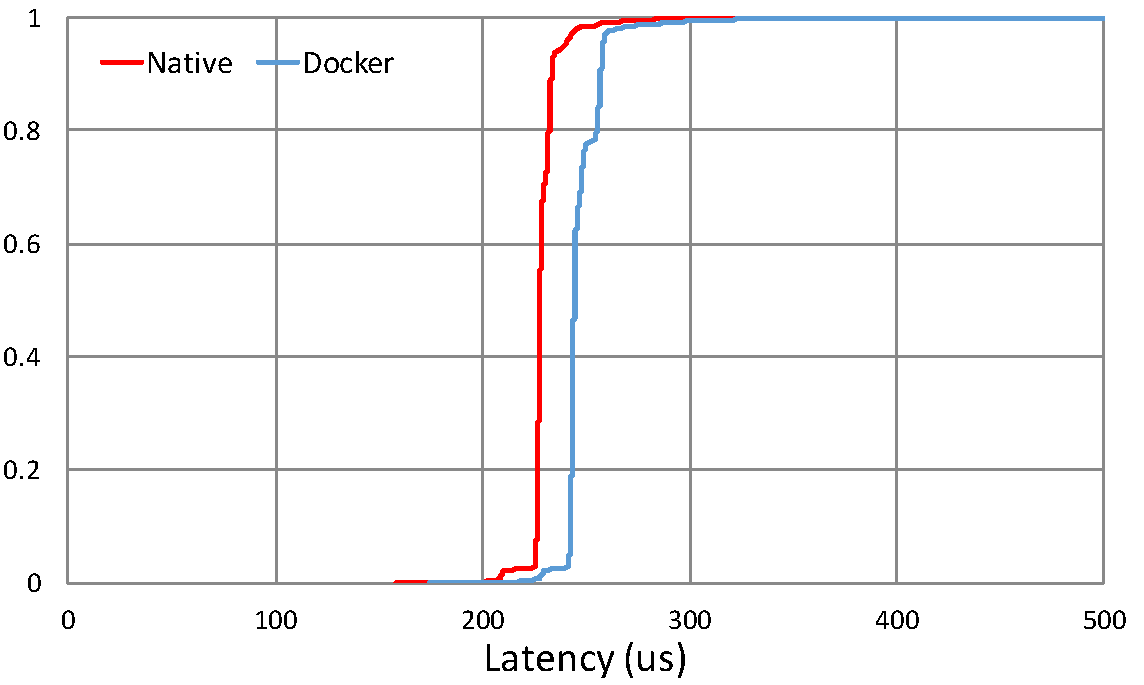
\includegraphics[height=1.8in, width=3in]{cpucdf.pdf}
\caption{The CDF of latency using bare metal and Docker container}
\label{fig:cpucdf}
\end{figure}

\begin{table}
\centering
\caption{Latency measurements of bare metal and Docker container}
\label{tbl:cpubase}
\begin{tabular}{|l|c|c|c|} \hline
$$& \textbf{mean(us)} & \textbf{median(us)} & \textbf{p99(us)}\\ \hline
\textbf{Bare metal} & 240.7 & 241.0 & 278.0 \\ \hline
\textbf{Docker container} & 255.2 & 255.0 & 295.0 \\ \hline\end{tabular}
\end{table}

\subsubsection{Case 1: Using CPU Shares}

We run the server process with `\textbf{--cpuset-cpus=``3''}' setting to realize CPU affinity and the `\textbf{--cpu-shares=1024}' as a default setting in CFS scheduler. Assume that two containers have different shares and are running on the same CPU core and `\textbf{--cpu-shares=1024}' is set. Container A has a share of 1,024 and container B has a share of 512, if both containers are CPU-intensive, which means they take almost all the time to do CPU calculation. The CPU time used by container A and container B would be at a ratio of 1024 : 512, which is 2 : 1. We run the test for 10 times. Each time 1,000,000 requests are transmitted between client and server. The CDF result is shown as the blue line in Figure \ref{fig:cpucdf}, and the mean, median and $99^{th}$-percentile position of the measurements are also listed in Table \ref{tbl:cpubase}.

From the above two test cases, we observe that when using Docker, the CPU latency almost shares the same CDF curve as using bare metal, except a little bias showing an additional fixed amount cost for CPU. Comparing both from the $99^{th}$-percentile column in Table \ref{tbl:cpubase} and the CDF curves in \ref{fig:cpucdf}, Docker container does not have a significant impact on the tail latency performance when using CPU shares. Just like mentioned in the report of IBM, Docker containers do have impact on CPU performance. However, the degradation is very low, 4\% in IBM's report about throughput and about 6\% about the mean, median, and $99^{th}$-percentile performance in our research. We conclude that when running CPU-intensive applications in a Docker container, the performance effect would be very small. Unlike VMs, which use hardware-level virtualization technology, Docker container's instructions do not need to be emulated by VMM. However, Docker containers share the same Linux kernel and use the same instructions as the host machine. An x86 instruction needs to be translated to several instructions to run on an ARM CPU using VMs. With the help of equation \ref{eq:vmsv}\cite{menasce2005virtualization}, we can do a rough calculation of the virtualization slowdown, where $f_p$ stands for the fraction of privileged instructions executed by a VM and $N_e$ stands for the average number of instructions required by the VMM to emulate a privileged instruction. The reason why Docker containers bring about a slightly slowdown is because when performing CPU isolation and limitation, the kernel needs to first check the namespace of the running process, thus the additional instructions would cause the extra latency.

\begin{equation}
\label{eq:vmsv}
S_v = f_p \times N_e + (1 - f_p)
\end{equation}

\subsubsection{Case 2: Using CPU Quota}

Apart from `\textbf{--cpu-shares}', there exist other parameters which limit the resource usage of CPU. `\textbf{--cpu-period}' means the period for the processes in the Docker container to be scheduled on the CPU. It is often used together with `\textbf{--cpu-quota}'  parameter. The unit of these two parameters are both microseconds. When these parameters are set, it means that processes in the container can use no more than `\textbf{--cpu-quota}' time during each `\textbf{--cpu-period}' time duration. To test whether these two parameters would have the same side effect as `\textbf{--cpu-shares}' when only one container is assigned to a CPU core, it can take all the cycles of that CPU, we carry out the following experiment:

\begin{table*}
\centering
\caption{Measurements of latency using `\textbf{--cpu-period}' and `\textbf{--cpu-quota}'}
\label{tbl:cpuperiod}
\begin{tabular}{|r|r|r|r|r|r|} \hline
\textbf{quota(us)} & \textbf{mean(us)} & \textbf{median(us)} & \textbf{p99(us)} & \textbf{\# $>$ 1,000us} & \textbf{\# $\times$ quota}\\ \hline
\textbf{1000} & 1035.4 & 307.0 & 7556.0 & 104996 & 104996000\\ \hline
\textbf{1500} & 579.5 & 258.0 & 5816.0 & 68221 & 102331500\\ \hline
\textbf{2000} & 489.0 & 281.0 & 4765.0 & 50187 & 100374000\\ \hline
\textbf{2500} & 361.7 & 260.0 & 3232.0 & 37334 & 93335000\\ \hline
\textbf{3000} & 291.9 & 259.0 & 1741.0 & 14273 & 42819000\\ \hline
\textbf{4000} & 258.0 & 253.0 & 331.0 & 39 & 156000\\ \hline
\textbf{5000} & 263.2 & 255.0 & 341.0 & 0 & 0\\ \hline
\textbf{7000} & 256.7 & 250.0 & 341.0 & 0 & 0\\ \hline
\textbf{10000} & 262.6 & 255.0 & 333.0 & 0 & 0\\ \hline
\end{tabular}
\end{table*}

We first fix `\textbf{--cpu-period=10000}' and vary the value of `\textbf{--cpu-quota}' to see the relationship between these two parameters. We choose values 1,000, 1,500, 2,000, 2,500, 3,000, 4,000, 5,000, 7,000, 10,000 for `\textbf{--cpu-quota}' and observe the results. These parameters are chosen because the minimum value of both these parameters are 1,000, and the magnitude gap is also set small. For each test, it is performed for 1,000,000 requests. We measure the mean, median, and $99^{th}$-percentile of the latencies. We also take the number of requests whose latency is greater than 1,000 us, the minimum time slice, into consideration. These results are shown in Table \ref{tbl:cpuperiod}. 

From Table \ref{tbl:cpuperiod}, we observe that latency increases incredibly when CPU quota only counts for a small ratio of the total CPU period. From 1,000 to 4,000, all mean, median and $99^{th}$-percentile are decreasing and so is the number of test cases whose latency is greater than 1,000 us. Figure \ref{fig:cpuquo} also shows the relationship between `\textbf{--cpu-quota}' and the number of requests whose latency is greater than 1,000 us. From this picture, we can see that the number first drops fast and then slowly as quota increases. When quota reaches over 3,000 us, latency suddenly drops fast and finally goes to about zero at 4,000.

\begin{figure}
\centering
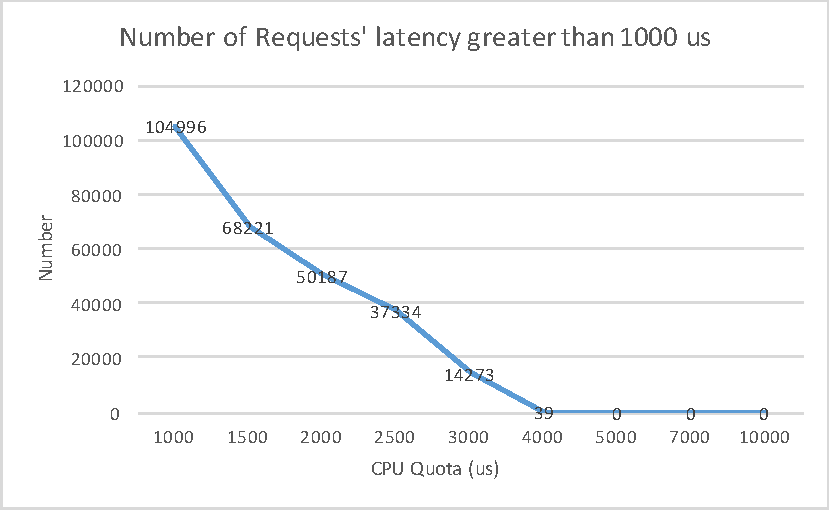
\includegraphics[height=1.6in, width=3in]{cpu_quota.pdf}
\caption{Number of requests' latency beyond 1 ms}
\label{fig:cpuquo}
\end{figure}

Unlike using CPU share, once only a single process is using the CPU, it can take all the CPU resources, using CPU period together with CPU quota options has a force cut off when the CPU usage is over the limited number. Since the client is calling the server continuously, once a request has finished, another request will immediately follows. If the server process uses up its quota during one period, it is sure to give up the CPU and wait until the next period comes. This can cause a very long tail latency in real time services, which is shown as a sudden rise in the $99^{th}$-percentile. Once the service is CPU-intensive or being visited quickly, it will add unwilling latency to the service, thus reducing the overall performance.

To prove the above theory, we first compute the last column in Table \ref{tbl:cpuperiod}. Assume we need in total time $t_{cpu}$ to do all the computation, which means the total time the process is running on CPU. CPU quota is $t_q$, and CPU period is $t_p$. Total number of requests blocked by the CPU options $n$ is computed as follows: $n = t_{cpu} / t_q$. Thus, total time $t_{total}$ needed to compute all the requests is: $t_{total} = n \times t_p$. So once $t_{cpu}$ is determined, we can see that $n \times t_p = t_{cpu}$ is also determined. In our experiment, we assume the CPU time cost for each request is $t_{request}$, and the total number of requests is $r$. So we see that $t_{cpu} = t_{request} \times r$ is determined, and $n \times t_q$ must be also determined, which is shown as the last column in our experiment. We can observe that for the case 1000, 1500, 2000, 2500, the products are around 100,000,000, which satisfy our formula. However, when $t_q$ comes to over 3000, the product falls incredibly. This phenomenon occurs because at this time, $t_q$ is greater than the overall CPU used. We use \textit{htop} command to measure CPU usage and the CPU use rate of that CPU is around 30\%. This is the reason why it suddenly falls at the 3000 point, which has $3000 / 10000 = 30\%$, and then quickly goes to 0. We also see from Figure \ref{fig:cpuquo} that when it comes to over 4000, the mean, median and  $99^{th}$-percentile are almost not affected, which means that when the CPU usage of the application is less than the ratio of quota to period, it has low impact on the latency performance.

\subsubsection{CPU Interference}

There is no meaning running a single process on a CPU core while at the same time limiting its available CPU resources. In the real world Docker cloud, if the CPU resources allocated to a container is very limited and less than one CPU core, sharing a single core among many containers can not be avoided. Once a latency sensitive container is allocated such configurations of resources, then there is a urgent need to know the interference between the newly added container and the existing latency sensitive one.

In this experiment, server side is hold in a container on CPU \#3 of the server host machine. Server uses `\textbf{--net=host}' to eliminate the interference of Linux bridge. Client side is also hold on a dedicated CPU on the client machine, while not inside a container. The client continuously ping the server using Apache Thrift, while at the same time no additional data is transmitted between the two processes except for the necessary Apache Thrift overhead. Although the server container is authorized to use all the memory and network resources, since we are focusing on the CPU interference of Docker containers, CPU quota is limited. We fix CPU period 10000 us not changed among all the experiments. On the other hand, CPU quota is varying from 5000 us to 9000 us for the server container. At the same time, another container is running on the same CPU as the server container. This container is continuously running a matrix multiplication process. The matrix multiplication involves two 512 x 512 matrixes. In each iteration, we log down the execution time. The sum of the CPU quotas of the matrix container together with the latency container is equals to the CPU period container. For example, if the CPU quota of latency container is 9000 us, then that of matrix container is $10000 - 9000 = 1000 us$.

\subsection{Network Isolation}

In this experiment, server sends or receives various length data to or from the client. We choose message sizes 1KB, 10KB, 30KB, 50KB, 70KB and100KB.  All message sizes are chosen from \textit{SPECWeb2009}\cite{specweb2009commerce} as the standard web message sizes. We test 1 million requests for each experiment.

Sever is hosted in a Docker container on one machine and client is running natively on another machine. Both server and client are assigned to a dedicated CPU to reduce performance interference. We compare two Docker configurations, the first one is to use `\textbf{--net=host}', which means the container directly use the host network port and the network isolation mechanism is not working. The second one is to use `\textbf{-p portA:portB}', which means container uses Linux bridge to communicate to the outside world. The \textbf{portA} used by the container is mapped to \textbf{portB} of the host machine, and it's working similar to the $NAT$ mechanism\cite{tsirtsis2000network}.

\subsubsection{Case 1: Server Receives Data}

In this case, client sends data to server using RPC calls and pass data through string parameters. We compare the mean, median and $99^{th}$-percentile result between using `\textbf{--net=host}' and `\textbf{-p portA:portB}'. Results are shown in Figures \ref{fig:recv}(a-c).

\begin{figure*}[!htb]
  \centering 
  \subfigure[Receive: Mean]{ 
    \label{fig:recva} %% label for first subfigure 
    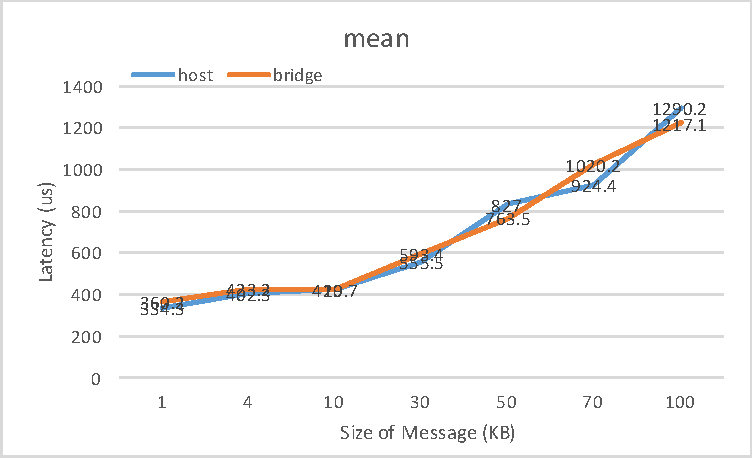
\includegraphics[width=2.2in,height=1.3in]{recv_a.pdf}} 
  %\hspace{0.3in} 
  \subfigure[Receive: Median]{ 
    \label{fig:recvb} %% label for second subfigure 
    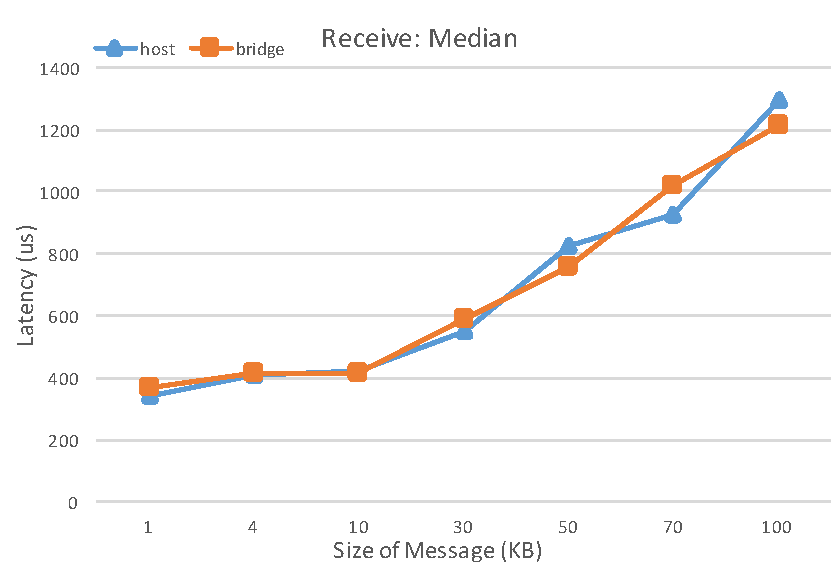
\includegraphics[width=2.2in,height=1.3in]{recv_b.pdf}} 
  %\hspace{0.3in} 
  \subfigure[Receive: $99^{th}$-percentile]{ 
    \label{fig:recvc} %% label for second subfigure 
    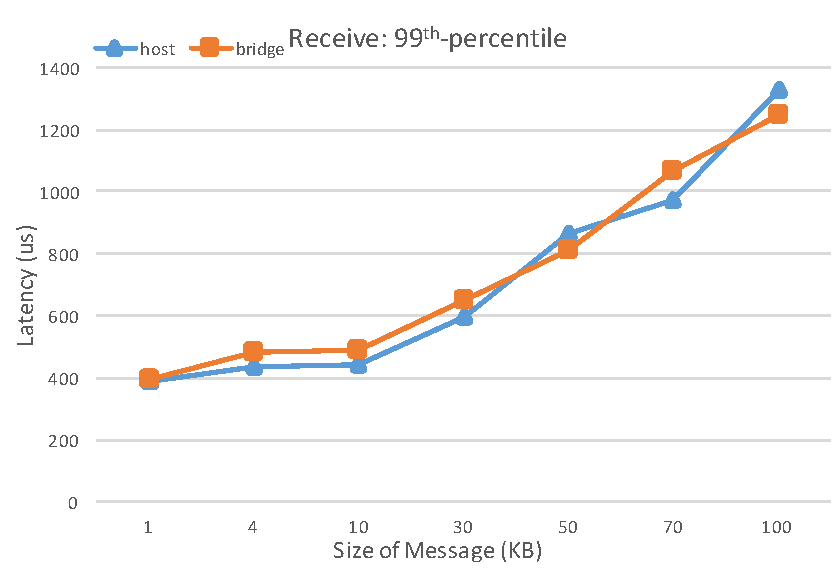
\includegraphics[width=2.2in,height=1.3in]{recv_c.pdf}} 
    \subfigure[Send: Mean]{ 
    \label{fig:senda} %% label for first subfigure 
    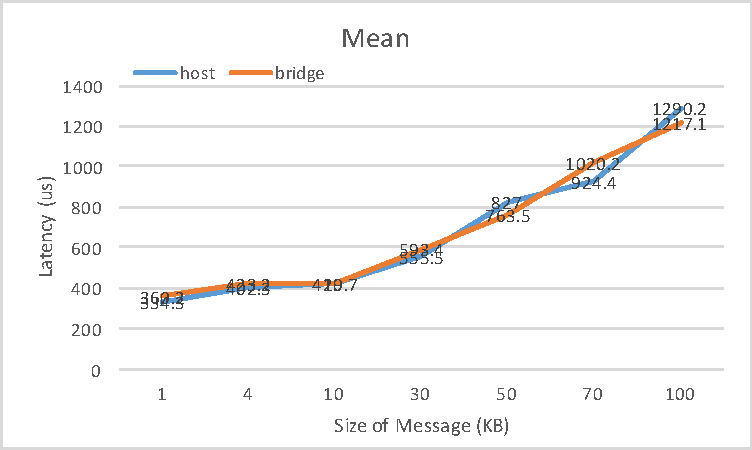
\includegraphics[width=2.2in,height=1.3in]{send_a.pdf}} 
  %\hspace{0.3in} 
  \subfigure[Send: Median]{ 
    \label{fig:sendb} %% label for second subfigure 
    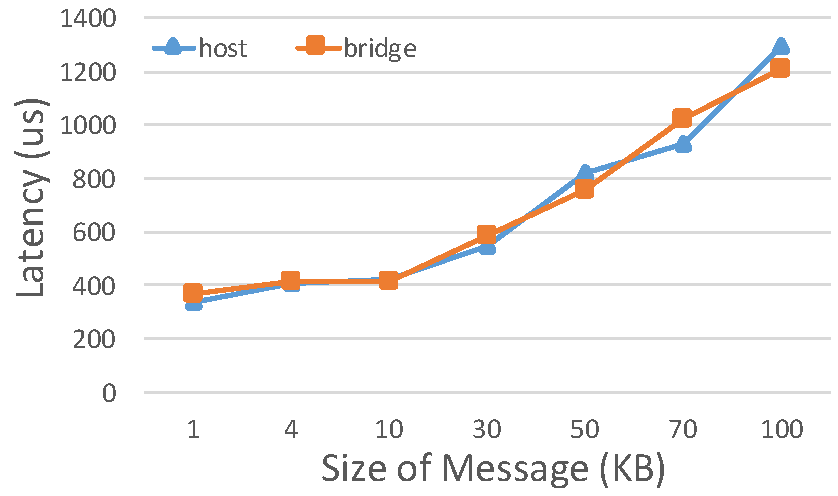
\includegraphics[width=2.2in,height=1.3in]{send_b.pdf}} 
  %\hspace{0.3in} 
  \subfigure[Send: $99^{th}$-percentile]{ 
    \label{fig:sendc} %% label for second subfigure 
    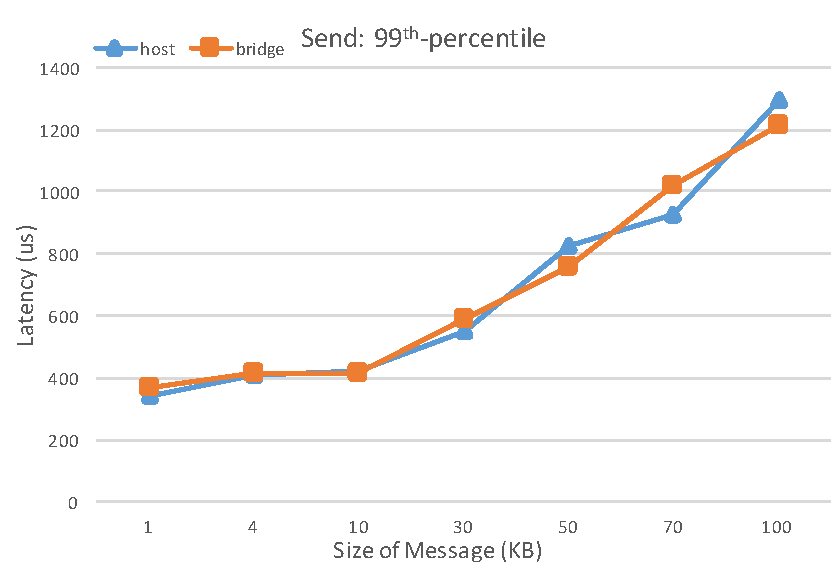
\includegraphics[width=2.2in,height=1.3in]{send_c.pdf}} 
  \caption{Mean, median, and $99^{th}$-percentile latency when server receive and send data.} 
  \label{fig:recv} %% label for entire figure 
\end{figure*}

\subsubsection{Case 2: Server Sends Data}

This time, client calls server with a single parameter indicating size and server returns the corresponding size string. Results similar to Section 3.3.1 are shown in Figures \ref{fig:recv}(d-f).

\subsubsection{Analysis}

As is shown in both figures, most of latencies using `\textbf{-p portA:portB}' are no more than 110\% of latencies using `\textbf{--net=host}' in each size group. In fact, when file size becomes much larger, the results are  very close to each other, and the slowdown percentage is nearly zero. Some of the comparison groups even witness a phenomenon where Docker bridge outperforms Docker host. This is because many other factors could slightly change the latency, including CPU scheduling, preempting, network contention, etc. They are outside the scope of this study.

However, according to IBM, there is a 80\% slowdown using Docker bridge\cite{felter2015updated}. So why our experiment draws a totally different result from IBM's research? There are several reasons. First, from our observation of the experiment, the degradation is `one-time'. It only adds a fixed latency to each trip. In our experiment, when the size of message is small, the impact of this fixed latency becomes large -- nearly 10\%. However, when message size is much larger, the impact of this latency is negligible, and the random vibration takes the dominance of the difference.

In IBM's report, it uses docker on both server and client side, which means a single round trip message goes through bridges four times, each side two. While in our experiment, it only happens at server side and totally two times. IBM's report uses 100B and 200B message size, while messages used in our experiment are much larger. Also, we use python and Thrift, which add much extra cost to the CPU and network, so the baseline might be much larger than in IBM's report. The size 0 situation is over 200 us as shown in the CPU experiment section. While all latencies in IBM's report are less than 100us. So we can not simply describe the impact of Docker bridge on the network performance as a percentage slowdown. It is a fixed-length degradation.

To understand the fixed-length degradation, we dive into the source code of Linux bridge. Taking the receive stage as an example, when a message has arrived at the NIC, it is uploaded to the upper layer in the network stack. It first checks whether this message is used by more than one application or it is to be multicasted. If not, it does no process including large amount of data copy. If so, the message is copied several times and then sent to each receiver, thus costing huge amount of extra latency. However, apparently in our experiment and IBM's experiment, the message is only used by a single application, without multicasting. Also, the message transmission is done by transferring a pointer to the message. So these extra functions will only cause a fixed extra time. This is why it affect so much in IBM's report while in ours slightly.

\subsection{File Operations Using AUFS}

Many applications like SQL server and Hadoop involve disk I/O operations. Disk operation latency of Docker container is thus another issue we should care about. In this experiment, only one application is hosted in a Docker container. The application continuously writes content of different sizes to a file. The length written each time are 1KB, 4KB, 10KB, 30KB, 50KB, 70kB, and 100KB. We compare two situations, the first one is to directly write messages inside the container, while the second is to write messages to a file outside and mounted to the container using `\textbf{-v}' option. To make sure that the messages are written to the disk immediately instead of staying in the cache area, each time we write a single message, we will use the `\textbf{flush()}' function to force the system to flush messages onto the disk. In each experiment group, the application continuously write 10,000 times and we repeat this operation for 10 times. We only discuss about the write case instead of the read one to avoid the pre-read situation where blocks of files are read in advance. We note down the mean, median and $99^{th}$-percentile measurements. The results are shown in Figure \ref{fig:write}.

\begin{figure*}[!htb]
  \centering 
  \subfigure[Mean]{ 
    \label{fig:recva} %% label for first subfigure 
    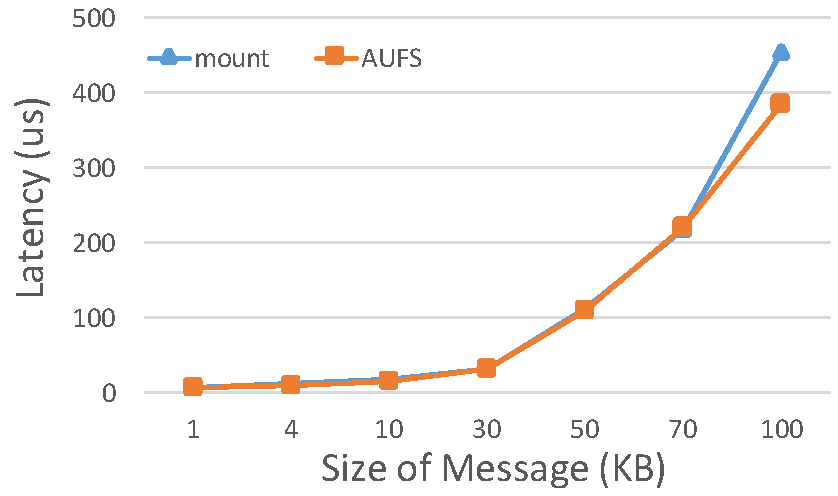
\includegraphics[width=2.2in,height=1.3in]{write_a.pdf}} 
  %\hspace{0.3in} 
  \subfigure[Median]{ 
    \label{fig:recvb} %% label for second subfigure 
    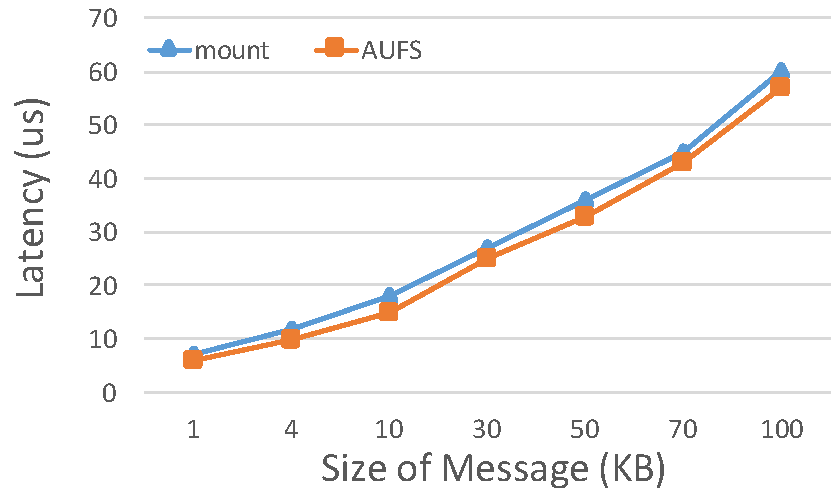
\includegraphics[width=2.2in,height=1.3in]{write_b.pdf}} 
  %\hspace{0.3in} 
  \subfigure[$99^{th}$-percentile]{ 
    \label{fig:recvc} %% label for second subfigure 
    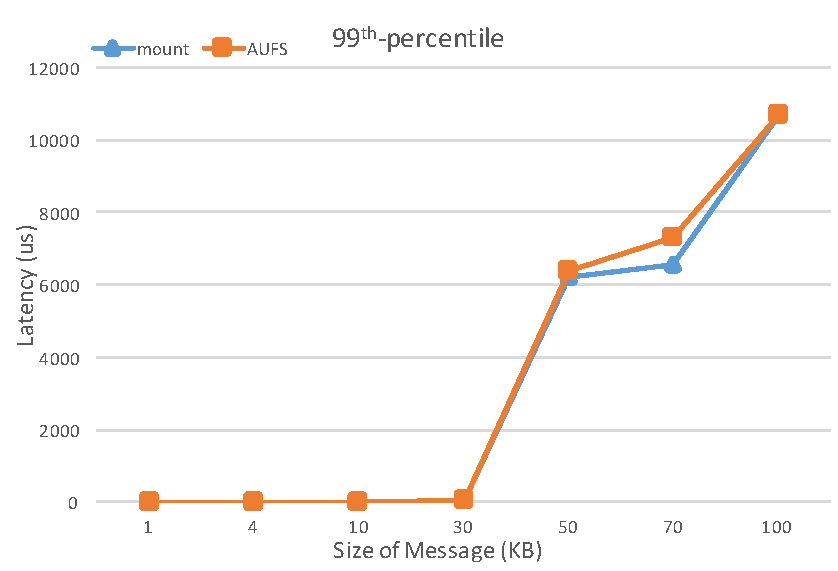
\includegraphics[width=2.2in,height=1.3in]{write_c.pdf}} 
  \caption{Mean, median, and $99^{th}$-percentile file write latency using mount and AUFS.} 
  \label{fig:write} %% label for entire figure 
\end{figure*}

From Figure \ref{fig:write}, we can observe that there is almost no impact on performance using AUFS when writing files. This result is the same as the one drawn from IBM's disk I/O report. This phenomenon is explained as follows. When a file is open, due to the copy-on-write feature of AUFS, a new file is created to hide the original file and a pointer to this file is returned to the application. The following operations are just like the normal operations on a disk file, and there is no fix-length latency degradation as in the network case.

\begin{figure}
\centering
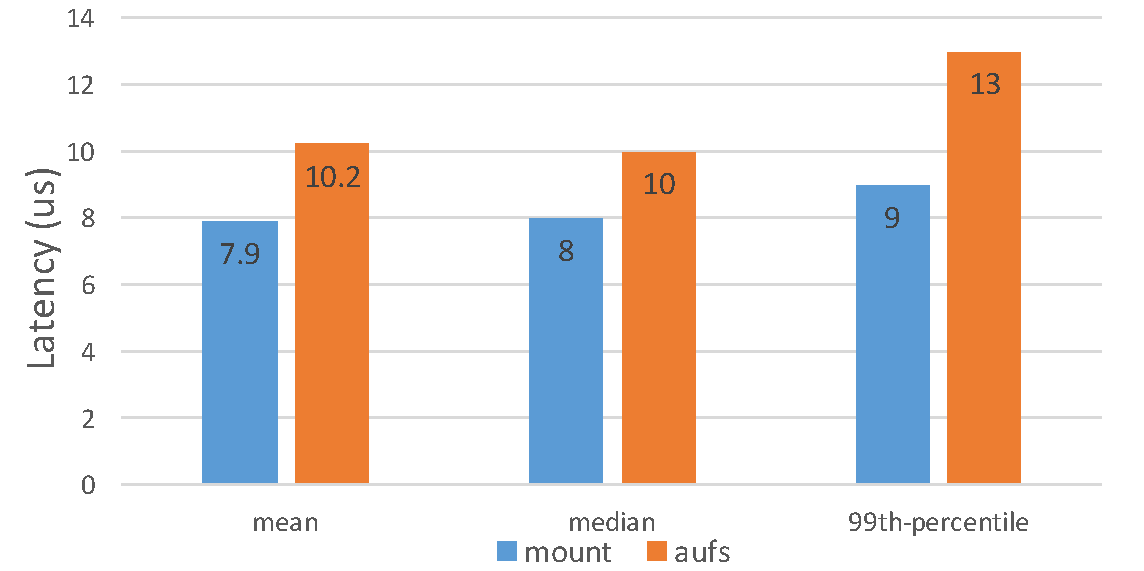
\includegraphics[height=1.5in, width=3in]{open.pdf}
\caption{Latency Comparison between mount and AUFS when opening a file}
\label{fig:open}
\end{figure}

However, there are cases reported that operating on files involves a significant performance degradation. Considering the feature of AUFS, we guess that the latency lies in the operation of opening a file. To confirm our guess, we carry out another group of experiment where the application continuously open and close a file 1,000,000 times. We note down the time required to open the file and the comparison is shown in Figure \ref{fig:open}.



From Figure \ref{fig:open}, we can find that there is a huge difference between using mount and AUFS concerning the open time of a file. This is because when using AUFS, since a Docker container is implemented combining several layers together, it must perform several additional functions to decide which layer the file is in. Sometimes it even has to copy another version of an existing file to perform the copy-on-write operation. These costs are huge compared to the time to open a file on the bare metal. Also, when first time writing to an existing file in the container, the larger the original file is, the longer the operation latency will be, which is caused by the cost of copy-on-write feature.


Building an image over another is a very convenient feature of Docker. You can simply add some files or run `\textbf{apt get}' command to install applications to the new image. All modifications are done in a new copy-on-write layer based on the original image layers. If a new file share the same name as an existing file, the original file will be hidden and only the newly added file can be seen by user. 

Just like open operations which take extra time due to locating the file in multiple layers, programs like `\textbf{ls}' which involve traversing the directory have to go through unneeded hidden files. To prove this, we build images from the official \textbf{ubuntu} image. Each time a new image is built, we add linux kernel source code directory (53.9MB) to the \textbf{/home} directory of the previous image. We build 32 such images, each has a new linux kernel source code directory located in \textbf{/home} hiding the original directory. In each directory, we run the `\textbf{time ls -R /home > > /dev/null}' command to note down the time consumption. Each experiment is done 100 times and we choose the mean measurement of the results. The outputs are shown in Figure \ref{fig:layer}. It is easy to observe from the figure that with the increment of the number of layers, latency is increasing too. Also, the line is almost linear except for some vibration. This might because the \textbf{ls -R} command will go through each layer of the \textbf{/home} directory. The reason why intercept is not zero is because the additional cost of output messages to \textbf{/dev/null} and there exists branch cut in each scan of the hidden layer to avoid too much additional time cost.

\begin{figure}
\centering
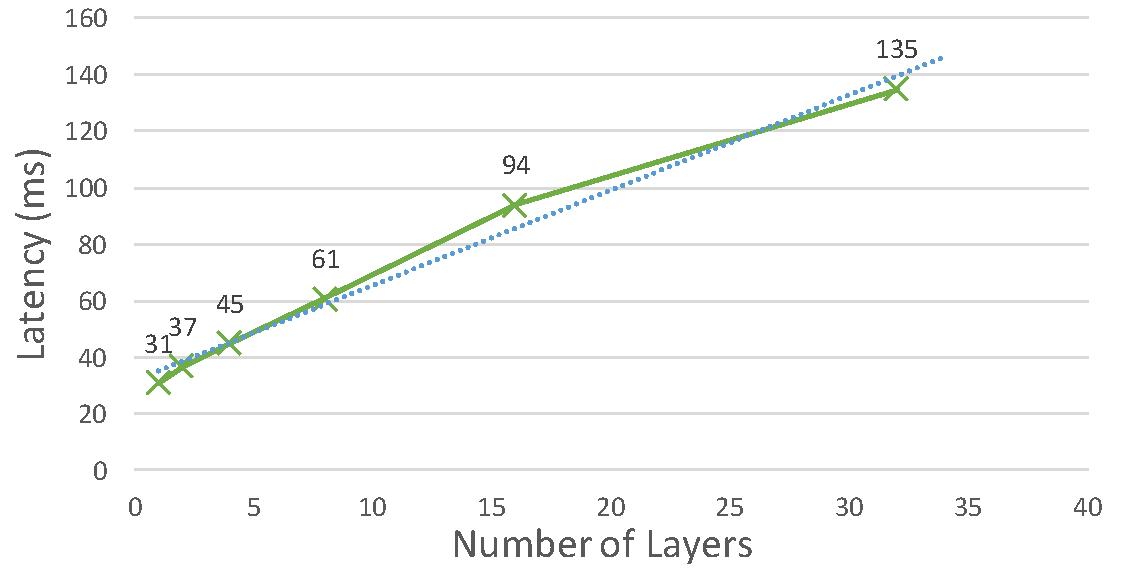
\includegraphics[height=1.5in, width=3in]{layer.pdf}
\caption{\textbf{ls -R} latency measurement}
\label{fig:layer}
\end{figure}

Docker provides a method to flatten the images. Although this method is originally meant to erase the hidden files in the low layers and decrease the number of layers (the total number of layers is limited to 42 originally and it becomes to 127 recently), it does some help in this situation. The recommended method to build a new image is to write a \textbf{Dockerfile}. However, Docker provides us with other methods to build a new image. These are two commands \textbf{save} and \textbf{export}. All these commands are acted on a running container instead of images. For example, if we execute the \textbf{save} command on a running container, all files in the lower layers and the current running layer will be saved to a \textbf{.tar} local file. If we use the \textbf{import} to save the original file as a new image, we would find that the layers' tree structure of the image is still saved using the \textbf{--tree} option. On the other hand, if we use the \textbf{export} command, and again import the newly created \textbf{.tar} file to a new image, we would find that there is only one layer left. This means that all the layers are flattened to a single layer, and if there are hidden files, the hidden files are thrown from the image. Only the ones you can see in a container are left. Also, the original image size of the one containing 32 layers of Linux source files is 1.911 GB. The one with only one layer of Linux source files is 241.8 MB. If we flatten an image with 32 layers of Linux source files, we would find the new one is 241.6 MB. The two values are very close but slightly different. So where does this 0.2 MB go? This is easy to explain. If we compress both the original \textbf{ubuntu} image and also the image with one layer of Linux source files, we find that both these two new images are shrinking with a size of 0.2 MB. Actually, the original \textbf{ubuntu} images is composed of many layers, and there also exists opportunities to compress this image.

In the following experiment, we flatten all the created images from one additional layer of Linux source files and 32 layers of Linux source files. We also execute the \textbf{ls -R} command in the Linux source file tree to note down the execution time for 100 times each image. We choose the average measurement as the final result. These results are shown in Figure. From Figure , we can find that the line is almost horizontal. Also, the execution time is just very close to the one as the original image with only one additional layer of Linux source files. So we can conclude that there is no extra time wasted on scanning the hidden files when the original image is flattened.

Since this method is so fascinating, is there any additional cost? Just like building a new image will involve huge amount of time, actually, there is. We log down the additional time to export the running image and create a new one, which is shown in Figure. To our surprise, the additional cost is not very high -- less than 10 seconds! Although there exists a linear increment as the number of layers increases, the execution time of the 32 layers situation is rather close to that of the one layer situation. This additional time consumption is very cheap in deploying a new service. Another drawback is that the new image is not based on old images and we can not make use of the layer structure to save disk storage. However, disk storage is almost the cheapest one nowadays and programmers usually don't mind much about the extra cost. We can even believe that the saved execution time and the increased service quality will overwhelm the extra cost of the additional start time.

\section{Conclusion and Discussions}

Docker is not so real-time-latency-friendly. Although \textbf{--cpu-shares} is a good choice as it doesn't cause a huge tail latency, in public cloud, many applications share a single CPU, using \textbf{--cpu-shares} can lead to a single application consumes more CPU than it is allowed to use when other applications are not running on this CPU. This is good for the consumers, but not fair since a consumer enjoys more resources than he has paid. Also, when service providers continuously allocate and de-allocate containers on a CPU, applications running on that core will go through performance vibrations. While using \textbf{--cpu-quota}, it is suitable for those CPU intensive works like many scientific workflow and HPC applications\cite{xavier2013performance}, but not those real time interactive services due to the possible long tail latency. 

Docker assumes that users traditionally run applications on a desktop version of Linux, and thus enable the CFS while disable the real time one. There are two way to let the servers have this additional real-time feature. The first one is to add options for Docker to support real-time scheduling. The other is more difficult but brings a lot good -- implement another scheduling that takes both throughput and real time performance into consideration, and we won't need to reboot the machine to change the setting of CPU scheduler.

Many applications involve small size of messages, like Redis Cache\cite{zawodny2009redis} and NoSQL databases\cite{strauch2011nosql}. When using Linux bridge to transmit message, it takes much more additional time due to short message size and high throughput, thus reducing the overall performance. But for applications like web gallery, since a photo is usually more than 1MB, the fix-length latency slowdown is overwhelmed by the system vibration, thus being less important in these cases. When using Linux bridge together with small size messages, it's not so latency-friendly since the extra time consumption is relatively large. We hope that a new method of transmitting information between Docker containers on different machines can be implemented to reduce this overall latency.

Some applications include many file operations. If the application simply open several big files one time and continuously write and read them, then we can neglect the disk I/O overhead since operating an open file using AUFS is just like natively. However, if the application involves huge number of file open operations, it can cause a huge extra latency (over 20\%). So applications running in Docker should not incorporate too many open operations and sometimes the design of the application has to be changed to suit Docker, thus bringing the programmers a lot of trouble.

Another thing we should bare in mind when using Docker is to reduce overall layers. Operations like traversing the file system involves going through hidden files in the low layers of AUFS, and we don't need these useless additional cost. One way to avoid this is to merge the different layers together and delete unnecessary files, either at container start time or image build time. However, additional time would be needed to merge the layers at these two stages. But these time are usually tolerable.

\section{Future Works}

Many future works can be done to reduce the latency and address the performance bottleneck. The first way is that Docker contributors taking action. Just as we mentioned above, to reduce the tail latency caused by Docker, contributors can add the support for real-time scheduling algorithms to provide customers with more choice. Also, the current CPU quota granularity is not so real-time friendly. Since in our test most of the latencies are below 1000 us, and the smallest CPU quota is 1000 us, we would usually meet the situation where a service has used up its quota and waiting for the remaining period, thus Linux CGroups can employ lower CPU quota granularity. Docker can also take the priority to monitor all the containers on a host machine. Once it finds a container's CPU consumption behavior looks like a real-time one, it can give this container lower CPU quota granularity to satisfy the real-time demand. It can also increase the priority of the real-time container. Once a new request from users has come, the service can immediate preempt the CPU and quickly return the result, while at the same time, the upper bound of the CPU cost of this container is also limited. A more interesting method is to let Docker daemon dynamically allocate resources when the containers are running. It can move those real-time containers on certain CPUs and left other used for those CPU intensive ones. Docker can then do optimizations on separate CPUs to let containers perform that. Since monitoring containers will cost host machine additional resources, cloud service suppliers can let the customers state their inclination before deploying services, and suppliers can then move the containers to the most suitable host machine. However, customers don't always choose the best configurations and thus expose the potential problem that customers' services perform terribly and various type of containers interfere the performance of each other.

In the case of network latency, Docker is performing very bad and even falls behind KVM \cite{felter2015updated}. This long latency is caused by the overhead of Linux bridge. So the latency problem can be solved by simply discard Linux bridge and write Docker's own network stack. However, there is almost no opportunities for Docker network to perform exactly the same as using Docker host. Additional operations will always exist to provide network isolation and security between containers.

For the additional cost of file operations, there are several situations for Docker to improve. The first is to add the support for flatting at the container start time. However, this will add additional startup cost and containers may not so outperform virtual machines in start time. In another method, we don't flatten the container at start time. Once the application in the container has scanned some directories, the scanned directories are flatten. Although the first execution would be time consuming, the following operations on the same directory will be much faster. The above two methods are just like the difference between C++ and C\#. The former involves compiling the file in advance and the second employs the method of just-in-time compilation.

Unfortunately, all above latency related questions of Docker are not solved currently. Cloud service customers can not wait until the new features of Docker come true. Then it is the customers' responsibility to take these extra latency into consideration. Customers can buy a cloud machine, and configure the containers themselves. As we have mentioned above, sending a large trunk of data once a time will reduce the effect of the extra fix-length latency. Thus many kinds of works are suitable for this case. Image bed, which is a storage system dedicated for photos, store and transmit images. Most of the images are very large (usually more than 1 MB) and we can fully make use of the size to narrow down the performance effect of network latency. Hadoop map-reduce applications are also suitable for this work since the files to be mapped and reduced are transmitted in the unit of trunk and these trunks are usually no less than 64 MB. If the application in a Docker container is some kind of database, we recommend that applications which interact with these databases transmit large amount of data once at a time. This can be done by predicting the users' requests and preload data from the database. It can also be done by merging several requests together and query the database once to reach all these data. Fetching a lot of small size data separately can lead to a significant performance degradation as stated in the MySQL performance test of IBM report.

Another suggestion for service suppliers is to add new files instead of modify existing files. If we have to modify a 1 GB file, we have to copy the file and then operate on the newly created file due to the AUFS's copy-on-write feature. This can lead to two problems. The first problem is that the copy process will bring about huge slow start latency, while the other lies in the wasted disk storage. For those applications which can not avoid open many existing files in the low layers, a solution is to open these needed files when application start and avoid to close them during execution. This can lead to a slow application start time but increase the following operations' performance. However, due to the limited memory resource and valuable file descriptors, the limitation of this method is also obvious: you can not open two much files at a time. The best method to solve the traverse latency problem is to flatten the images in advance. However, this cannot solve the file open latency problem, since even if the image is flattened, you are still operating on a lower layer and can never avoid the copy-on-write process. But it does reduce some latency since there is no need for file system to scan the unneeded hidden layers. 

A very serious problem of Docker containers is their security issues. People are working hard to address these problems. Docker contributors are trying to increase the security level of current Docker containers while maintain their current light-weight feature. However, this work is not that easy since Docker employs many Linux kernel technologies. An increment in the level of security and isolation can include the modification of kernel, which is hard to be done and difficult to be applied to all operating systems running a container. Another method comes from the opposite side. We can make the existing virtual machines more light-weight while still remain the isolation and security capability. There are methods that run containers in virtual machines, however, this is totally unnecessary and ridiculous since applications have to go through the cost of two additional layers. The security and isolation level is no better than using only virtual machine while overhead incredibly increases. So we should think of other methods to combine virtual machines and containers together. VSphere Integrated Containers (VIC) is a new container technology provided by VMWare. Although it employs hardware-level virtualization, which can lead to worse performance than light-weight containers, it provides users with better isolation and security. It is also far different from traditional virtual machines since it provides the concept of images and layers. Although it doesn't have the performance advantage over containers, it takes the easy-to-deploy feature of Docker into consideration and provides better deployment experience for programmers. 


%\section{Not Mine}
%
%The \textit{proceedings} are the records of a conference.
%ACM seeks to give these conference by-products a uniform,
%high-quality appearance.  To do this, ACM has some rigid
%requirements for the format of the proceedings documents: there
%is a specified format (balanced  double columns), a specified
%set of fonts (Arial or Helvetica and Times Roman) in
%certain specified sizes (for instance, 9 point for body copy),
%a specified live area (18 $\times$ 23.5 cm [7" $\times$ 9.25"]) centered on
%the page, specified size of margins (1.9 cm [0.75"]) top, (2.54 cm [1"]) bottom
%and (1.9 cm [.75"]) left and right; specified column width
%(8.45 cm [3.33"]) and gutter size (.83 cm [.33"]).
%
%The good news is, with only a handful of manual
%settings\footnote{Two of these, the {\texttt{\char'134 numberofauthors}}
%and {\texttt{\char'134 alignauthor}} commands, you have
%already used; another, {\texttt{\char'134 balancecolumns}}, will
%be used in your very last run of \LaTeX\ to ensure
%balanced column heights on the last page.}, the \LaTeX\ document
%class file handles all of this for you.
%
%The remainder of this document is concerned with showing, in
%the context of an ``actual'' document, the \LaTeX\ commands
%specifically available for denoting the structure of a
%proceedings paper, rather than with giving rigorous descriptions
%or explanations of such commands.
%
%\section{The {\secit Body} of The Paper}
%Typically, the body of a paper is organized
%into a hierarchical structure, with numbered or unnumbered
%headings for sections, subsections, sub-subsections, and even
%smaller sections.  The command \texttt{{\char'134}section} that
%precedes this paragraph is part of such a
%hierarchy.\footnote{This is the second footnote.  It
%starts a series of three footnotes that add nothing
%informational, but just give an idea of how footnotes work
%and look. It is a wordy one, just so you see
%how a longish one plays out.} \LaTeX\ handles the numbering
%and placement of these headings for you, when you use
%the appropriate heading commands around the titles
%of the headings.  If you want a sub-subsection or
%smaller part to be unnumbered in your output, simply append an
%asterisk to the command name.  Examples of both
%numbered and unnumbered headings will appear throughout the
%balance of this sample document.
%
%Because the entire article is contained in
%the \textbf{document} environment, you can indicate the
%start of a new paragraph with a blank line in your
%input file; that is why this sentence forms a separate paragraph.
%
%\subsection{Type Changes and {\subsecit Special} Characters}
%We have already seen several typeface changes in this sample.  You
%can indicate italicized words or phrases in your text with
%the command \texttt{{\char'134}textit}; emboldening with the
%command \texttt{{\char'134}textbf}
%and typewriter-style (for instance, for computer code) with
%\texttt{{\char'134}texttt}.  But remember, you do not
%have to indicate typestyle changes when such changes are
%part of the \textit{structural} elements of your
%article; for instance, the heading of this subsection will
%be in a sans serif\footnote{A third footnote, here.
%Let's make this a rather short one to
%see how it looks.} typeface, but that is handled by the
%document class file. Take care with the use
%of\footnote{A fourth, and last, footnote.}
%the curly braces in typeface changes; they mark
%the beginning and end of
%the text that is to be in the different typeface.
%
%You can use whatever symbols, accented characters, or
%non-English characters you need anywhere in your document;
%you can find a complete list of what is
%available in the \textit{\LaTeX\
%User's Guide}\cite{Lamport:LaTeX}.
%
%\subsection{Math Equations}
%You may want to display math equations in three distinct styles:
%inline, numbered or non-numbered display.  Each of
%the three are discussed in the next sections.
%
%\subsubsection{Inline (In-text) Equations}
%A formula that appears in the running text is called an
%inline or in-text formula.  It is produced by the
%\textbf{math} environment, which can be
%invoked with the usual \texttt{{\char'134}begin. . .{\char'134}end}
%construction or with the short form \texttt{\$. . .\$}. You
%can use any of the symbols and structures,
%from $\alpha$ to $\omega$, available in
%\LaTeX\cite{Lamport:LaTeX}; this section will simply show a
%few examples of in-text equations in context. Notice how
%this equation: \begin{math}\lim_{n\rightarrow \infty}x=0\end{math},
%set here in in-line math style, looks slightly different when
%set in display style.  (See next section).
%
%\subsubsection{Display Equations}
%A numbered display equation -- one set off by vertical space
%from the text and centered horizontally -- is produced
%by the \textbf{equation} environment. An unnumbered display
%equation is produced by the \textbf{displaymath} environment.
%
%Again, in either environment, you can use any of the symbols
%and structures available in \LaTeX; this section will just
%give a couple of examples of display equations in context.
%First, consider the equation, shown as an inline equation above:
%\begin{equation}\lim_{n\rightarrow \infty}x=0\end{equation}
%Notice how it is formatted somewhat differently in
%the \textbf{displaymath}
%environment.  Now, we'll enter an unnumbered equation:
%\begin{displaymath}\sum_{i=0}^{\infty} x + 1\end{displaymath}
%and follow it with another numbered equation:
%\begin{equation}\sum_{i=0}^{\infty}x_i=\int_{0}^{\pi+2} f\end{equation}
%just to demonstrate \LaTeX's able handling of numbering.
%
%\subsection{Citations}
%Citations to articles \cite{bowman:reasoning,
%clark:pct, braams:babel, herlihy:methodology, soltesz2007container},
%conference proceedings \cite{clark:pct} or
%books \cite{salas:calculus, Lamport:LaTeX} listed
%in the Bibliography section of your
%article will occur throughout the text of your article.
%You should use BibTeX to automatically produce this bibliography;
%you simply need to insert one of several citation commands with
%a key of the item cited in the proper location in
%the \texttt{.tex} file \cite{Lamport:LaTeX}.
%The key is a short reference you invent to uniquely
%identify each work; in this sample document, the key is
%the first author's surname and a
%word from the title.  This identifying key is included
%with each item in the \texttt{.bib} file for your article.
%
%The details of the construction of the \texttt{.bib} file
%are beyond the scope of this sample document, but more
%information can be found in the \textit{Author's Guide},
%and exhaustive details in the \textit{\LaTeX\ User's
%Guide}\cite{Lamport:LaTeX}.
%
%This article shows only the plainest form
%of the citation command, using \texttt{{\char'134}cite}.
%This is what is stipulated in the SIGS style specifications.
%No other citation format is endorsed or supported.
%
%\subsection{Tables}
%Because tables cannot be split across pages, the best
%placement for them is typically the top of the page
%nearest their initial cite.  To
%ensure this proper ``floating'' placement of tables, use the
%environment \textbf{table} to enclose the table's contents and
%the table caption.  The contents of the table itself must go
%in the \textbf{tabular} environment, to
%be aligned properly in rows and columns, with the desired
%horizontal and vertical rules.  Again, detailed instructions
%on \textbf{tabular} material
%is found in the \textit{\LaTeX\ User's Guide}.
%
%Immediately following this sentence is the point at which
%Table 1 is included in the input file; compare the
%placement of the table here with the table in the printed
%dvi output of this document.
%
%\begin{table}
%\centering
%\caption{Frequency of Special Characters}
%\begin{tabular}{|c|c|l|} \hline
%Non-English or Math&Frequency&Comments\\ \hline
%\O & 1 in 1,000& For Swedish names\\ \hline
%$\pi$ & 1 in 5& Common in math\\ \hline
%\$ & 4 in 5 & Used in business\\ \hline
%$\Psi^2_1$ & 1 in 40,000& Unexplained usage\\
%\hline\end{tabular}
%\end{table}
%
%To set a wider table, which takes up the whole width of
%the page's live area, use the environment
%\textbf{table*} to enclose the table's contents and
%the table caption.  As with a single-column table, this wide
%table will ``float" to a location deemed more desirable.
%Immediately following this sentence is the point at which
%Table 2 is included in the input file; again, it is
%instructive to compare the placement of the
%table here with the table in the printed dvi
%output of this document.
%
%
%\begin{table*}
%\centering
%\caption{Some Typical Commands}
%\begin{tabular}{|c|c|l|} \hline
%Command&A Number&Comments\\ \hline
%\texttt{{\char'134}alignauthor} & 100& Author alignment\\ \hline
%\texttt{{\char'134}numberofauthors}& 200& Author enumeration\\ \hline
%\texttt{{\char'134}table}& 300 & For tables\\ \hline
%\texttt{{\char'134}table*}& 400& For wider tables\\ \hline\end{tabular}
%\end{table*}
%% end the environment with {table*}, NOTE not {table}!
%
%\subsection{Figures}
%Like tables, figures cannot be split across pages; the
%best placement for them
%is typically the top or the bottom of the page nearest
%their initial cite.  To ensure this proper ``floating'' placement
%of figures, use the environment
%\textbf{figure} to enclose the figure and its caption.
%
%This sample document contains examples of \textbf{.eps} files to be
%displayable with \LaTeX.  If you work with pdf\LaTeX, use files in the
%\textbf{.pdf} format.  Note that most modern \TeX\ system will convert
%\textbf{.eps} to \textbf{.pdf} for you on the fly.  More details on
%each of these is found in the \textit{Author's Guide}.
%
%\begin{figure}
%\centering
%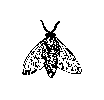
\includegraphics{fly}
%\caption{A sample black and white graphic.}
%\end{figure}
%
%\begin{figure}
%\centering
%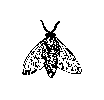
\includegraphics[height=1in, width=1in]{fly}
%\caption{A sample black and white graphic
%that has been resized with the \texttt{includegraphics} command.}
%\end{figure}
%
%
%As was the case with tables, you may want a figure
%that spans two columns.  To do this, and still to
%ensure proper ``floating'' placement of tables, use the environment
%\textbf{figure*} to enclose the figure and its caption.
%and don't forget to end the environment with
%{figure*}, not {figure}!
%
%\begin{figure*}
%\centering
%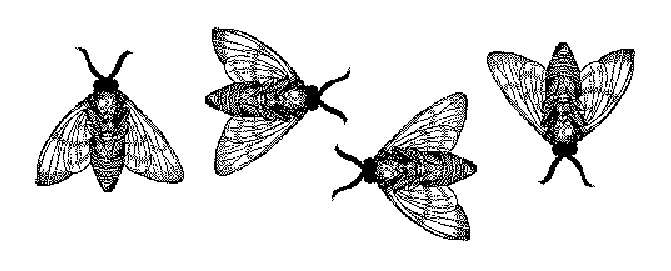
\includegraphics{flies}
%\caption{A sample black and white graphic
%that needs to span two columns of text.}
%\end{figure*}
%
%
%\begin{figure}
%\centering
%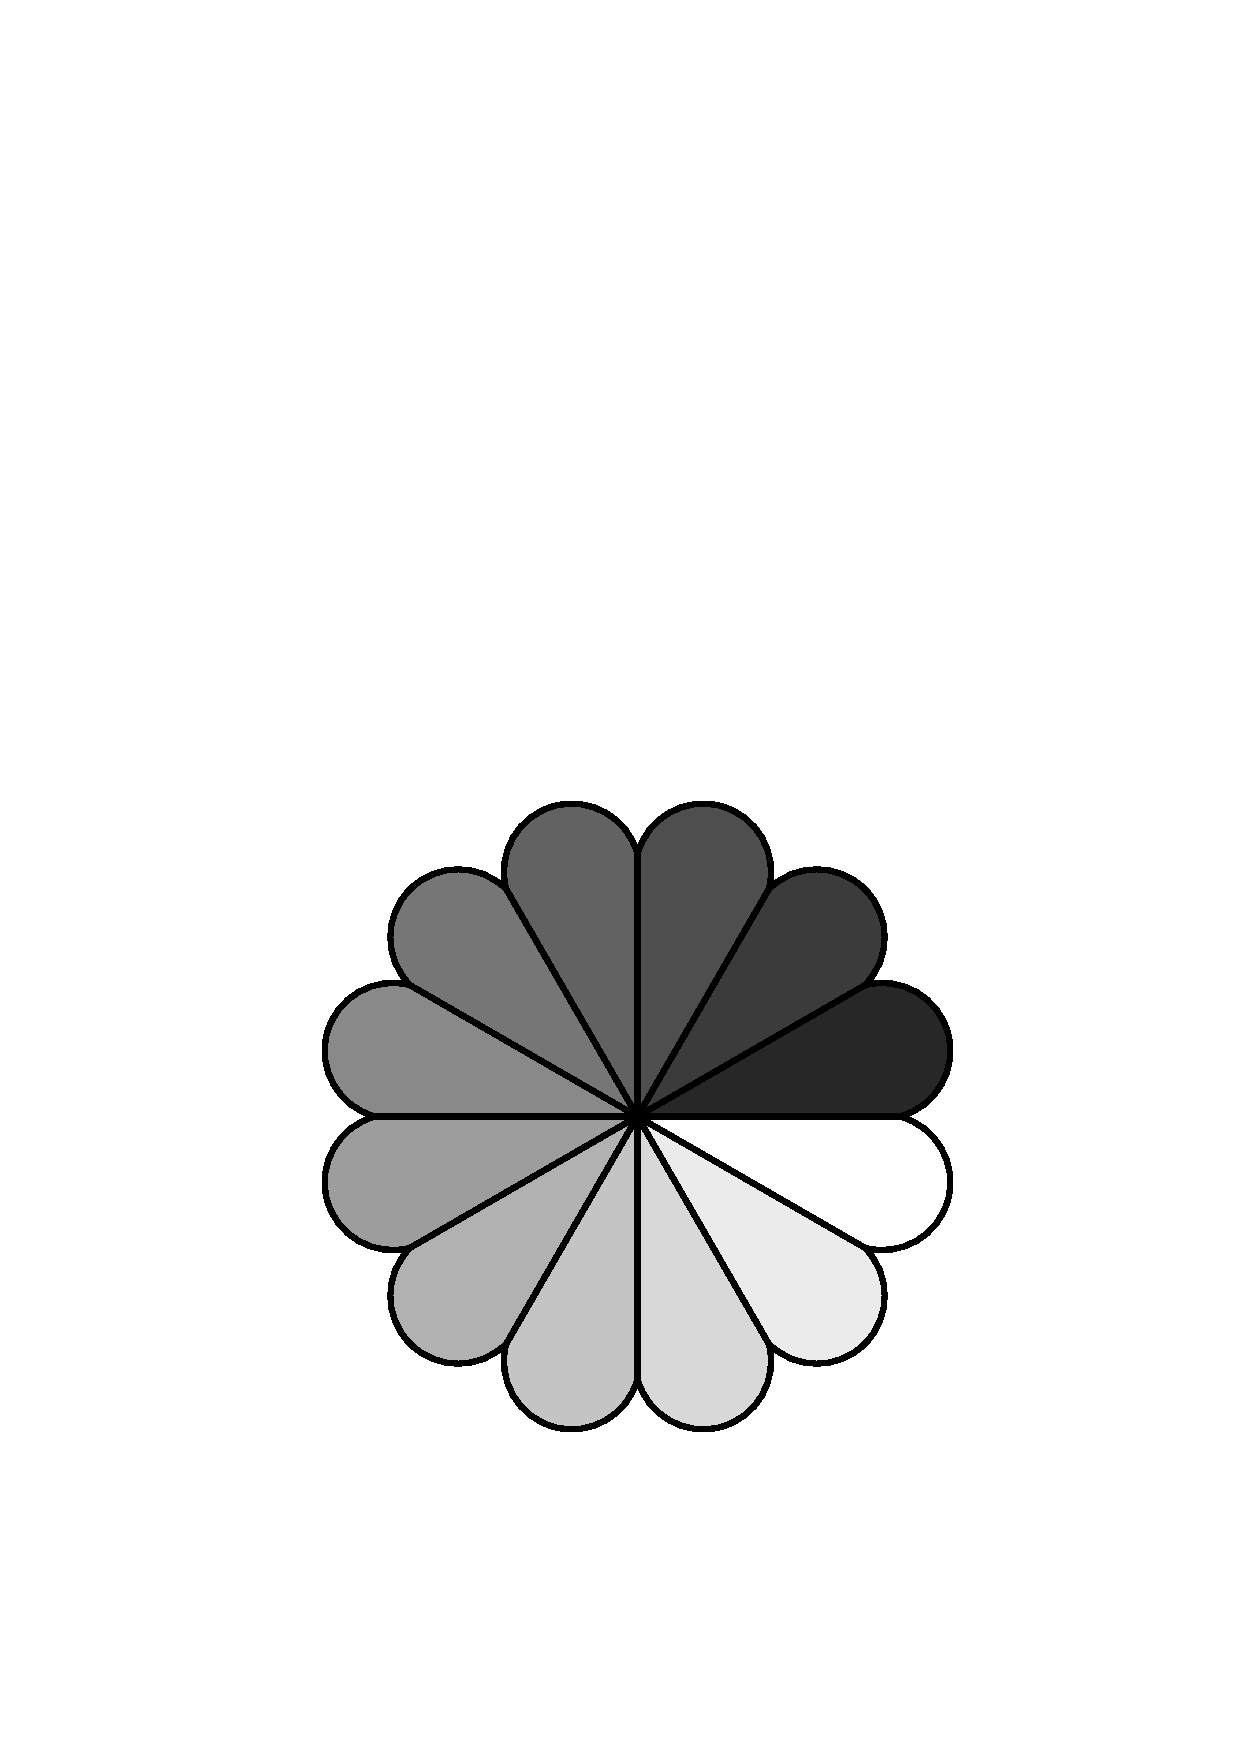
\includegraphics[height=1in, width=1in]{rosette}
%\caption{A sample black and white graphic that has
%been resized with the \texttt{includegraphics} command.}
%\vskip -6pt
%\end{figure}
%
%\subsection{Theorem-like Constructs}
%Other common constructs that may occur in your article are
%the forms for logical constructs like theorems, axioms,
%corollaries and proofs.  There are
%two forms, one produced by the
%command \texttt{{\char'134}newtheorem} and the
%other by the command \texttt{{\char'134}newdef}; perhaps
%the clearest and easiest way to distinguish them is
%to compare the two in the output of this sample document:
%
%This uses the \textbf{theorem} environment, created by
%the\linebreak\texttt{{\char'134}newtheorem} command:
%\newtheorem{theorem}{Theorem}
%\begin{theorem}
%Let $f$ be continuous on $[a,b]$.  If $G$ is
%an antiderivative for $f$ on $[a,b]$, then
%\begin{displaymath}\int^b_af(t)dt = G(b) - G(a).\end{displaymath}
%\end{theorem}
%
%The other uses the \textbf{definition} environment, created
%by the \texttt{{\char'134}newdef} command:
%\newdef{definition}{Definition}
%\begin{definition}
%If $z$ is irrational, then by $e^z$ we mean the
%unique number which has
%logarithm $z$: \begin{displaymath}{\log e^z = z}\end{displaymath}
%\end{definition}
%
%Two lists of constructs that use one of these
%forms is given in the
%\textit{Author's  Guidelines}.
% 
%There is one other similar construct environment, which is
%already set up
%for you; i.e. you must \textit{not} use
%a \texttt{{\char'134}newdef} command to
%create it: the \textbf{proof} environment.  Here
%is a example of its use:
%\begin{proof}
%Suppose on the contrary there exists a real number $L$ such that
%\begin{displaymath}
%\lim_{x\rightarrow\infty} \frac{f(x)}{g(x)} = L.
%\end{displaymath}
%Then
%\begin{displaymath}
%l=\lim_{x\rightarrow c} f(x)
%= \lim_{x\rightarrow c}
%\left[ g{x} \cdot \frac{f(x)}{g(x)} \right ]
%= \lim_{x\rightarrow c} g(x) \cdot \lim_{x\rightarrow c}
%\frac{f(x)}{g(x)} = 0\cdot L = 0,
%\end{displaymath}
%which contradicts our assumption that $l\neq 0$.
%\end{proof}
%
%Complete rules about using these environments and using the
%two different creation commands are in the
%\textit{Author's Guide}; please consult it for more
%detailed instructions.  If you need to use another construct,
%not listed therein, which you want to have the same
%formatting as the Theorem
%or the Definition\cite{salas:calculus} shown above,
%use the \texttt{{\char'134}newtheorem} or the
%\texttt{{\char'134}newdef} command,
%respectively, to create it.
%
%\subsection*{A {\secit Caveat} for the \TeX\ Expert}
%Because you have just been given permission to
%use the \texttt{{\char'134}newdef} command to create a
%new form, you might think you can
%use \TeX's \texttt{{\char'134}def} to create a
%new command: \textit{Please refrain from doing this!}
%Remember that your \LaTeX\ source code is primarily intended
%to create camera-ready copy, but may be converted
%to other forms -- e.g. HTML. If you inadvertently omit
%some or all of the \texttt{{\char'134}def}s recompilation will
%be, to say the least, problematic.
%
%\section{Conclusions}
%This paragraph will end the body of this sample document.
%Remember that you might still have Acknowledgments or
%Appendices; brief samples of these
%follow.  There is still the Bibliography to deal with; and
%we will make a disclaimer about that here: with the exception
%of the reference to the \LaTeX\ book, the citations in
%this paper are to articles which have nothing to
%do with the present subject and are used as
%examples only.
%\end{document}  % This is where a 'short' article might terminate

%ACKNOWLEDGMENTS are optional
%\section{Acknowledgments}
%This section is optional; it is a location for you
%to acknowledge grants, funding, editing assistance and
%what have you.  In the present case, for example, the
%authors would like to thank Gerald Murray of ACM for
%his help in codifying this \textit{Author's Guide}
%and the \textbf{.cls} and \textbf{.tex} files that it describes.

%
% The following two commands are all you need in the
% initial runs of your .tex file to
% produce the bibliography for the citations in your paper.
\bibliographystyle{abbrv}
\bibliography{sigproc}  % sigproc.bib is the name of the Bibliography in this case


% You must have a proper ".bib" file
%  and remember to run:
% latex bibtex latex latex
% to resolve all references
%
% ACM needs 'a single self-contained file'!
%
%APPENDICES are optional
%\balancecolumns
%\appendix
%%Appendix A
%\section{Headings in Appendices}
%The rules about hierarchical headings discussed above for
%the body of the article are different in the appendices.
%In the \textbf{appendix} environment, the command
%\textbf{section} is used to
%indicate the start of each Appendix, with alphabetic order
%designation (i.e. the first is A, the second B, etc.) and
%a title (if you include one).  So, if you need
%hierarchical structure
%\textit{within} an Appendix, start with \textbf{subsection} as the
%highest level. Here is an outline of the body of this
%document in Appendix-appropriate form:
%\subsection{Introduction}
%\subsection{The Body of the Paper}
%\subsubsection{Type Changes and  Special Characters}
%\subsubsection{Math Equations}
%\paragraph{Inline (In-text) Equations}
%\paragraph{Display Equations}
%\subsubsection{Citations}
%\subsubsection{Tables}
%\subsubsection{Figures}
%\subsubsection{Theorem-like Constructs}
%\subsubsection*{A Caveat for the \TeX\ Expert}
%\subsection{Conclusions}
%\subsection{Acknowledgments}
%\subsection{Additional Authors}
%This section is inserted by \LaTeX; you do not insert it.
%You just add the names and information in the
%\texttt{{\char'134}additionalauthors} command at the start
%of the document.
%\subsection{References}
%Generated by bibtex from your ~.bib file.  Run latex,
%then bibtex, then latex twice (to resolve references)
%to create the ~.bbl file.  Insert that ~.bbl file into
%the .tex source file and comment out
%the command \texttt{{\char'134}thebibliography}.
%% This next section command marks the start of
%% Appendix B, and does not continue the present hierarchy
%\section{More Help for the Hardy}
%The sig-alternate.cls file itself is chock-full of succinct
%and helpful comments.  If you consider yourself a moderately
%experienced to expert user of \LaTeX, you may find reading
%it useful but please remember not to change it.
%%\balancecolumns % GM June 2007
%% That's all folks!
\end{document}
